\chapter{Introdução}
\pagenumbering{arabic}

Todo currículo de ciência da computação no mundo inclui um curso sobre
estruturas de dados e algoritmos. Estruturas de dados são importantes; elas
melhoram a nossa qualidade de vida e até mesmo podem salvar vidas
rotineiramente. Muitas empresas multi-bilionárias foram construídas em torno de
estruturas de dados.

Como isso acontece? Se paramos para pensar sobre isso, percebemos que
interagimos constantemente com as estruturas de dados.
\begin{itemize}
	\item  Abrir um arquivo: As estruturas de dados do sistema de arquivos 
	\index{sistema de arquivos}% 
	são usadas para localizar as partes desse arquivo no disco para que possam ser
	recuperadas. Isso não é fácil; discos contêm centenas de milhões de blocos. O
	conteúdo do seu arquivo pode ser armazenado em qualquer um deles. 
	\item Procurar um contato em seu telefone: uma estrutura de dados é usada para
	procurar um número de telefone em sua lista de contatos 
	\index{lista de contatos}% 
	com base em informações parciais mesmo antes de terminar de discagem/digitação. Isso não é fácil; seu telefone pode conter informações sobre um
	grande número de pessoas --- todos os que você já contactou por telefone ou
	e-mail --- e seu telefone não tem um processador muito rápido ou muita memória.
	\item Fazer login na sua rede social 
	\index{rede social}%
	favorita: os servidores de rede usam suas informações de login para procurar as
	informações de sua conta. Isso não é fácil; as redes sociais mais populares têm
	centenas de milhões de usuários ativos.
	\item Fazer uma pesquisa na web:
	\index{pesquisa web}%
	O mecanismo de pesquisa usa estruturas de dados para encontrar as páginas da
	web que contêm seus termos de pesquisa. Isso não é fácil; há mais de 8,5 bilhões
	de páginas na Internet e cada página contém muitos termos de pesquisa em
	potencial.
	\item Telefone de serviços de emergência (1-9-0): 
	\index{serviços de emergência}\index{9-1-1}%
	A rede de serviços de emergência procura o seu número de telefone em uma
	estrutura de dados que mapeia números de telefone para endereços para que carros
	de polícia, ambulâncias ou caminhões de bombeiros podem ser enviados para lá sem
	demora. Isso é importante; a pessoa que faz a chamada pode não ser capaz de
	fornecer o endereço exato que eles estão chamando e um atraso pode significar a
	diferença entre a vida ou a morte.
\end{itemize}

\section{A Necessidade de Eficiência}

Na próxima seção, analisamos as operações suportadas pelas estruturas de dados
mais usadas. Qualquer pessoa com um pouco de experiência de programação verá que
essas operações não são difíceis de implementar corretamente. Podemos armazenar
os dados em uma matriz ou uma lista vinculada e cada operação pode ser
implementada iterando sobre todos os elementos da matriz ou lista e
possivelmente adicionando ou removendo um elemento.

Este tipo de implementação é fácil, mas não muito eficiente. Mas isso realmente
importa? Os computadores estão se tornando cada vez mais rápidos. Talvez a
implementação óbvia seja boa o suficiente. Vamos fazer alguns cálculos
aproximados para descobrir.

\paragraph{Número de operações:}  Imagine um aplicativo com um conjunto de dados
de tamanho moderado, digamos de um milhão ($10^6$) de itens. É razoável, na
maioria das aplicações, assumir que o aplicativo vai procurar cada item pelo
menos uma vez. Isso significa que podemos esperar fazer pelo menos um milhão
($10^6$) de pesquisas nesses dados. Se cada uma dessas $10^6$ inspeções 
inspecionar cada um dos $10^6$ itens, isto dá um total de
$10^6\times10^6=10^{12}$ (um trilhão) de inspeções.

\paragraph{Velocidade do processador:} No momento da escrita deste texto, mesmo
um computador desktop muito rápido não pode fazer mais de um bilhão ($10^9$) de
operações por segundo.\footnote{As velocidades do computador são, no máximo, de
	alguns gigahertz (bilhões de ciclos por segundo), e cada operação tipicamente
	leva alguns ciclos.}
Isto significa que esta aplicação tomará pelo menos $10^{12}/10^9=1000$
segundos, ou cerca de 16 minutos e 40 segundos. Dezesseis minutos é uma
eternidade no tempo do computador, mas uma pessoa pode estar disposta a aturar
isso (Se ele ou ela saiu para uma pausa para o café).

%Consider, now an application like the human genome project.  Completed in
%2003 (when computers were quite a bit slower than they are now), this
%was considered an extraordinary scientific accomplishment.  The human
%genome consists of 3 billion ($3\times 10^6$) base pairs. By our
%rough calculations, doing even a single search on this data would take
%3 seconds.  Doing a million searches would take $3$ million seconds,
%or roughly 34 days.  This is starting to get beyond reasonable.

\paragraph{Grandes conjuntos de dados:} Agora considere uma empresa como o
Google, 
\index{Google}%
que indexa mais de 8,5 bilhões de páginas da web. Pelo nossos cálculos, fazer
qualquer tipo de consulta sobre esses dados levaria pelo menos 8,5 segundos. Já
sabemos que não é esse o caso; pesquisas na web concluem em menos de 8,5
segundos, e fazemos consultas muito mais complicadas do que apenas perguntar se
uma determinada página está em sua lista de páginas indexadas. Atualmente, o
Google recebe aproximadamente $4.500$ consultas por segundo, o que significa que
elas exigem pelo menos $4.500\times 8.5=38.250$ servidores muito rápidos apenas
para manter-se.

\paragraph{A solução:} 
Esses exemplos nos dizem que as implementações óbvias de estruturas de dados não
se dimensionam bem quando o número de itens,
$\ensuremath{\ensuremath{\mathit{n}}}$, na estrutura de dados e o número de
operações, $m$, realizados na estrutura de dados são ambos grandes. Nestes
casos, o tempo (medido em, digamos, instruções de máquina) é aproximadamente
$#n#\times m$.

A solução, é claro, é organizar cuidadosamente os dados dentro da estrutura de
dados para que nem todas as operações exijam que todos os itens de dados sejam
inspecionados. Embora pareça impossível no início, veremos estruturas de dados
onde uma pesquisa requer apenas dois itens em média, independentemente do número
de itens armazenados na estrutura de dados. Em nosso computador de um bilhão de
instruções por segundo, levamos apenas $0.000000002$ segundos para pesquisar em
uma estrutura de dados contendo um bilhão de itens (ou um trilhão, ou um
quatrilhão, ou até mesmo um quintilhão de itens).

Também veremos implementações de estruturas de dados que mantêm os itens em uma
ordem específica, na qual o número de itens inspecionados durante uma operação
cresce muito lentamente em função do número de itens na estrutura de dados. Por
exemplo, podemos manter um conjunto ordenado de um bilhão de itens enquanto
inspecionamos no máximo 60 itens durante qualquer operação. Em nosso computador
de um bilhão de instruções por segundo, essas operações levam $0.00000006$
segundos cada.

O restante deste capítulo revisa brevemente alguns dos principais conceitos
utilizados ao longo do restante do livro. A \secref{interfaces} descreve as
interfaces implementadas por todas as estruturas de dados descritas neste manual
e deve ser considerada leitura obrigatória. As seções restantes discutem:
\begin{itemize}
	\item Alguma revisão matemática incluindo exponenciais, logaritmos, fatoriais,
	notação assintótica (big-O, às vezes usada no Brasil como grande-O ou O-grande), probabilidade e randomização;
	\item o modelo de computação; 
	\item correção, tempo de execução e espaço;
	\item uma visão geral do resto dos capítulos; e 
	\item o código de exemplo e as convenções de escrita.
\end{itemize}
Um leitor com ou sem um conhecimento nessas áreas pode facilmente ignorá-las
agora e voltar a elas mais tarde, se necessário.

\section{Interfaces}
\seclabel{interfaces}
Ao discutir estruturas de dados, é importante entender a diferença entre a
interface de uma estrutura de dados e sua implementação. Uma interface descreve
o que uma estrutura de dados faz, enquanto uma implementação descreve como a
estrutura de dados o faz.

Uma \emph{interface},
\index{interface}%
\index{tipo abstrato de dados|see{interface}}%
às vezes também chamada de \emph{tipo abstrato de dados}, define o conjunto de
operações suportado por uma estrutura de dados e a semântica, ou significado,
dessas operações. Uma interface não nos diz nada sobre como a estrutura de dados
implementa essas operações; ela fornece somente uma lista de operações
suportadas junto com especificações sobre quais tipos de argumentos cada
operação aceita e o valor retornado por cada operação.

Uma \emph{implementação} de estrutura de dados, por outro lado, inclui 
a representação interna da estrutura de dados, bem como as definições 
dos algoritmos que implementam as operações suportadas pela estrutura de dados. 
Assim, pode haver muitas implementações de uma única interface. 
Por exemplo, no \chapref{arrays}, veremos implementações da interface #Lista#
usando arrays e 
no \chapref{linkedlists} veremos implementações da interface #Lista# usando
estruturas de 
dados baseadas em ponteiro. Cada uma implementa a mesma interface, #Lista#, mas
de maneiras diferentes.

\subsection{As Interfaces #Fila# (Queue), #Pilha# (Stack) e #Deque#}

A interface de #Fila# representa uma coleção de elementos aos quais podemos
adicionar elementos e remover o próximo elemento. Mais precisamente, as
operações suportadas pela interface #Fila# são
\begin{itemize}
	\item #add(x)#: enfileira o valor #x# na #Fila#
	\item #remove()#: remove o próximo (enfileirado anteriormente) valor, #y#, da
	#Fila# e retorna #y#
\end{itemize}
Observe que a operação #remove()# não assume nenhum argumento. A disciplina de
enfileiramento da #Fila# decide qual elemento deve ser removido. Existem muitas
disciplinas de filas possíveis, a mais comum incluem FIFO, prioridade e LIFO.

Uma Fila \emph{FIFO (first-in-first-out)},
\index{fila FIFO}%
\index{fila!FIFO}%
ilustrada na 
\figref{queue}, remove os itens na mesma ordem em que foram adicionados, da
mesma 
forma que uma fila de uma caixa de supermercado. Este é o tipo mais comum de
#Fila#, de modo que o 
qualificador FIFO é muitas vezes omitido. Em outros textos, as operações
#add(x)# e #remove()# 
em uma fila FIFO são frequentemente chamadas de #enqueue(x)# e #dequeue()#,
respectivamente.

\begin{figure}
	\centering{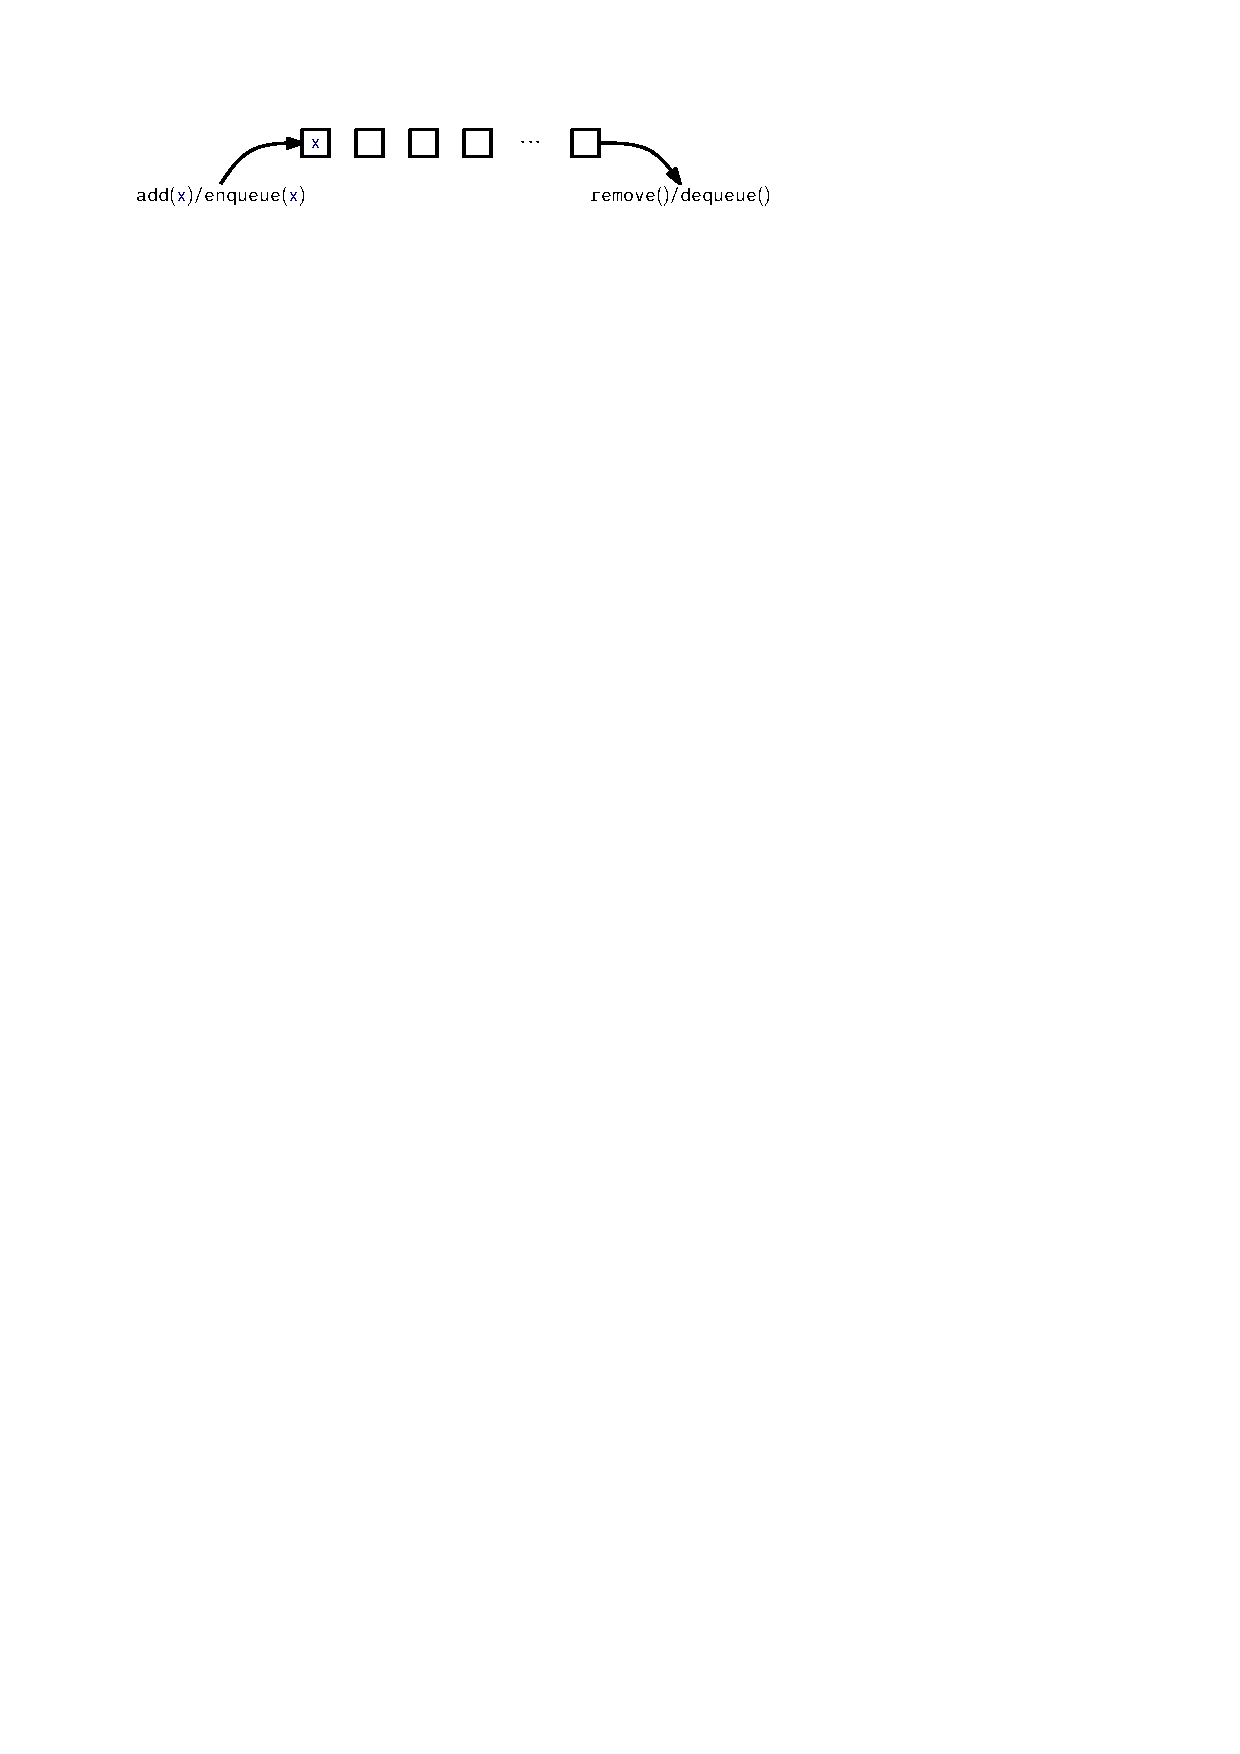
\includegraphics[width=\ScaleIfNeeded]{figs/queue}}
	\caption[Uma Fila FIFO]{Uma #Fila# FIFO.}
	\figlabel{queue}
\end{figure}

Uma \emph{Fila de prioridade},
\index{fila de prioridade}%
\index{fila de prioridade|seealso{heap}}%
\index{fila!prioridade}%
ilustrada na \figref{prioqueue}, sempre remove o menor elemento da #Fila#,
quebrando os laços arbitrariamente. Isto é semelhante à maneira pela qual é
feita a triagem de pacientes em uma sala de emergência do hospital. À medida que
os pacientes chegam, eles são avaliados e depois colocados em uma sala de
espera. Quando um médico se torna disponível, ele ou ela primeiro trata o
paciente com a condição mais fatal. A operação #remove()# em uma #Fila# de
Prioridade é normalmente chamada de #deleteMin()# em outros textos.

\begin{figure}
	\centering{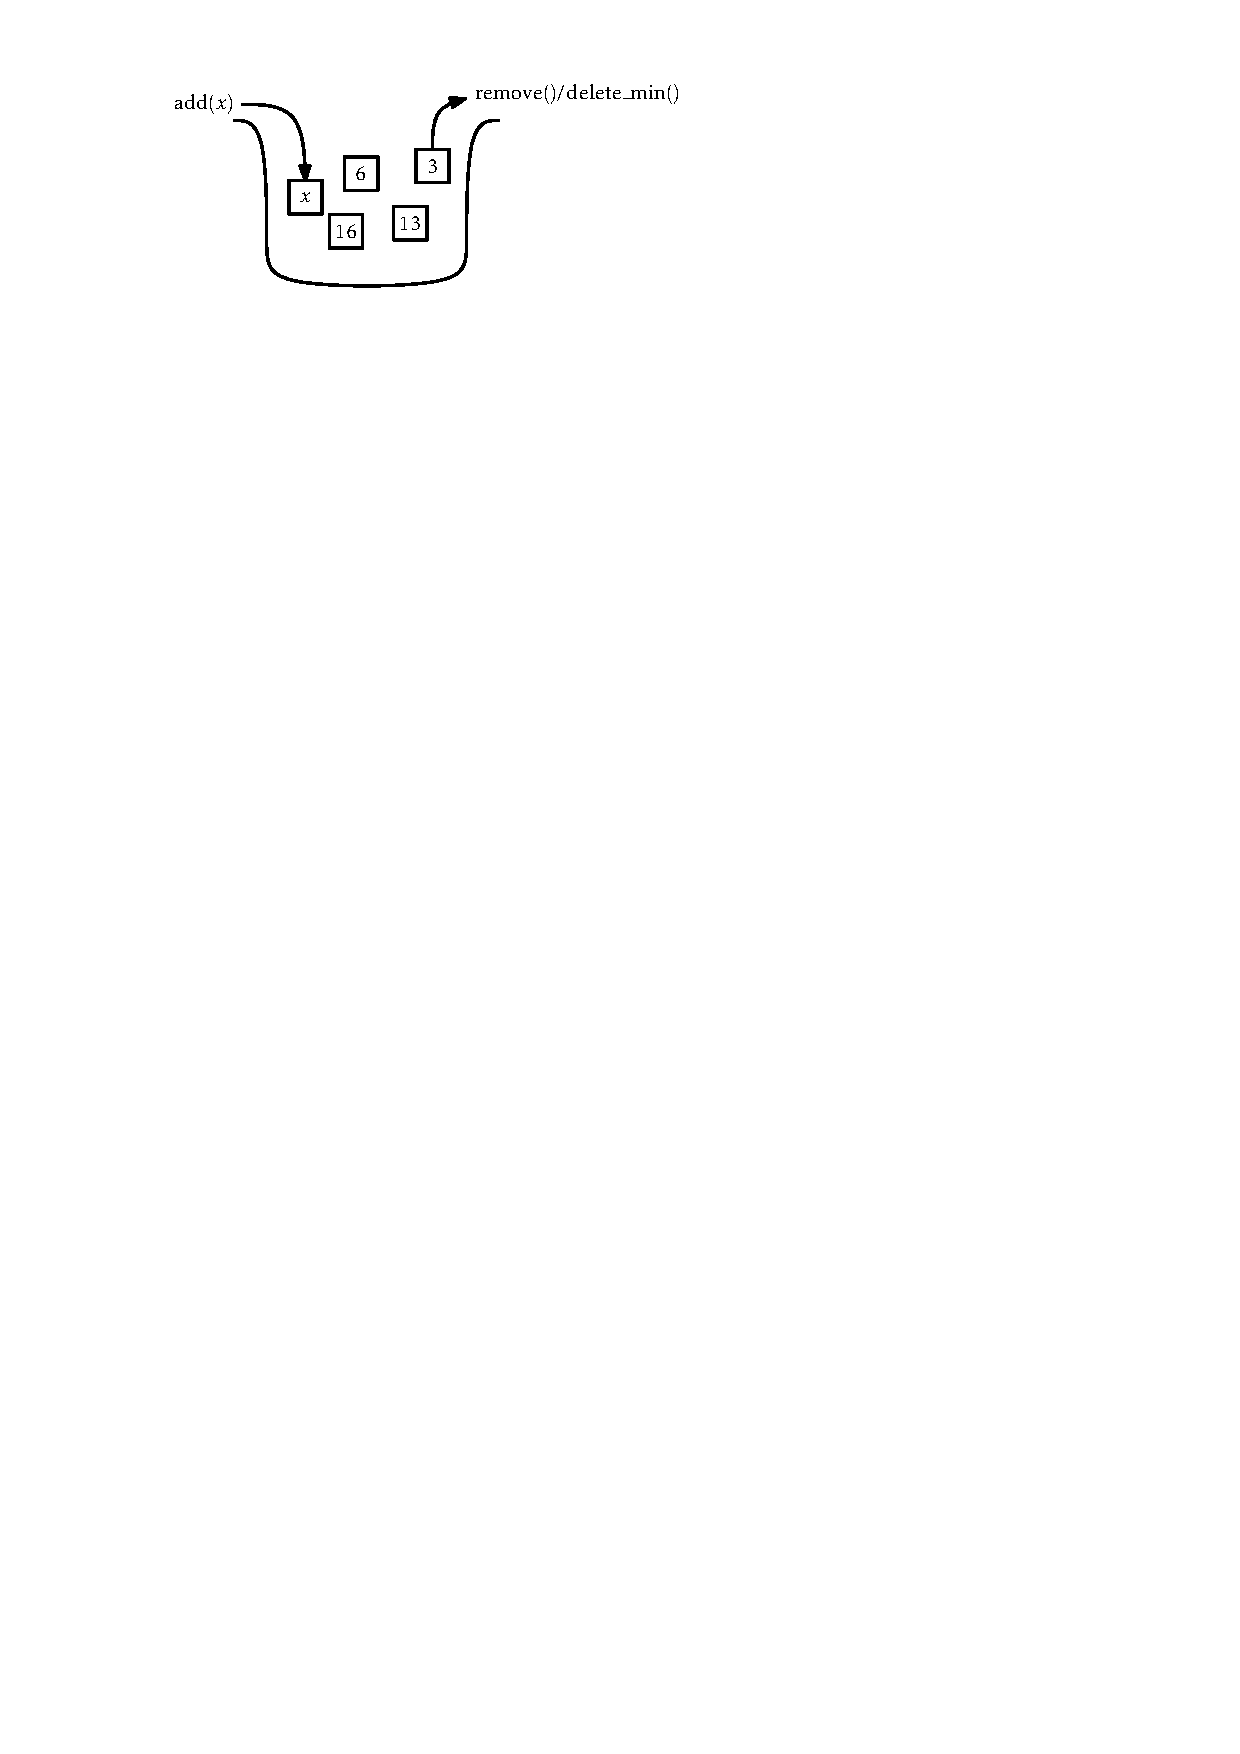
\includegraphics[width=\ScaleIfNeeded]{figs-python/prioqueue}}
	\caption[Uma #Fila# de Prioridade]{Uma Fila de Prioridade.}
	\figlabel{prioqueue}
\end{figure}

%This is similar to the way
%many airlines manage upgrades to the business class on their flights.
%When a business-class seat becomes available it is given to the most
%important customer waiting on an upgrade.

Uma disciplina de enfileiramento muito comum é a disciplina LIFO
(last-in-first-out), 
\index{fila LIFO}%
\index{fila LIFO|seealso{stack}}%
\index{fila!LIFO}%
\index{stack}%
ilustrada na \figref{stack}. Em uma \emph{Fila LIFO}, o elemento adicionado mais
recentemente é o próximo removido. Isto é melhor visualizado em termos de uma
pilha de pratos. Os pratos são colocados no topo da pilha e também removidos da
parte superior da pilha. Essa estrutura é tão comum que ele recebe seu próprio
nome: #Stack#. Muitas vezes, ao discutir uma #Stack#, os nomes de #add(x)# e
#remove()# são alterados para #push(x)# e #pop()#; isso é para evitar confundir
as disciplinas das filas LIFO e FIFO.


\begin{figure}
	\centering{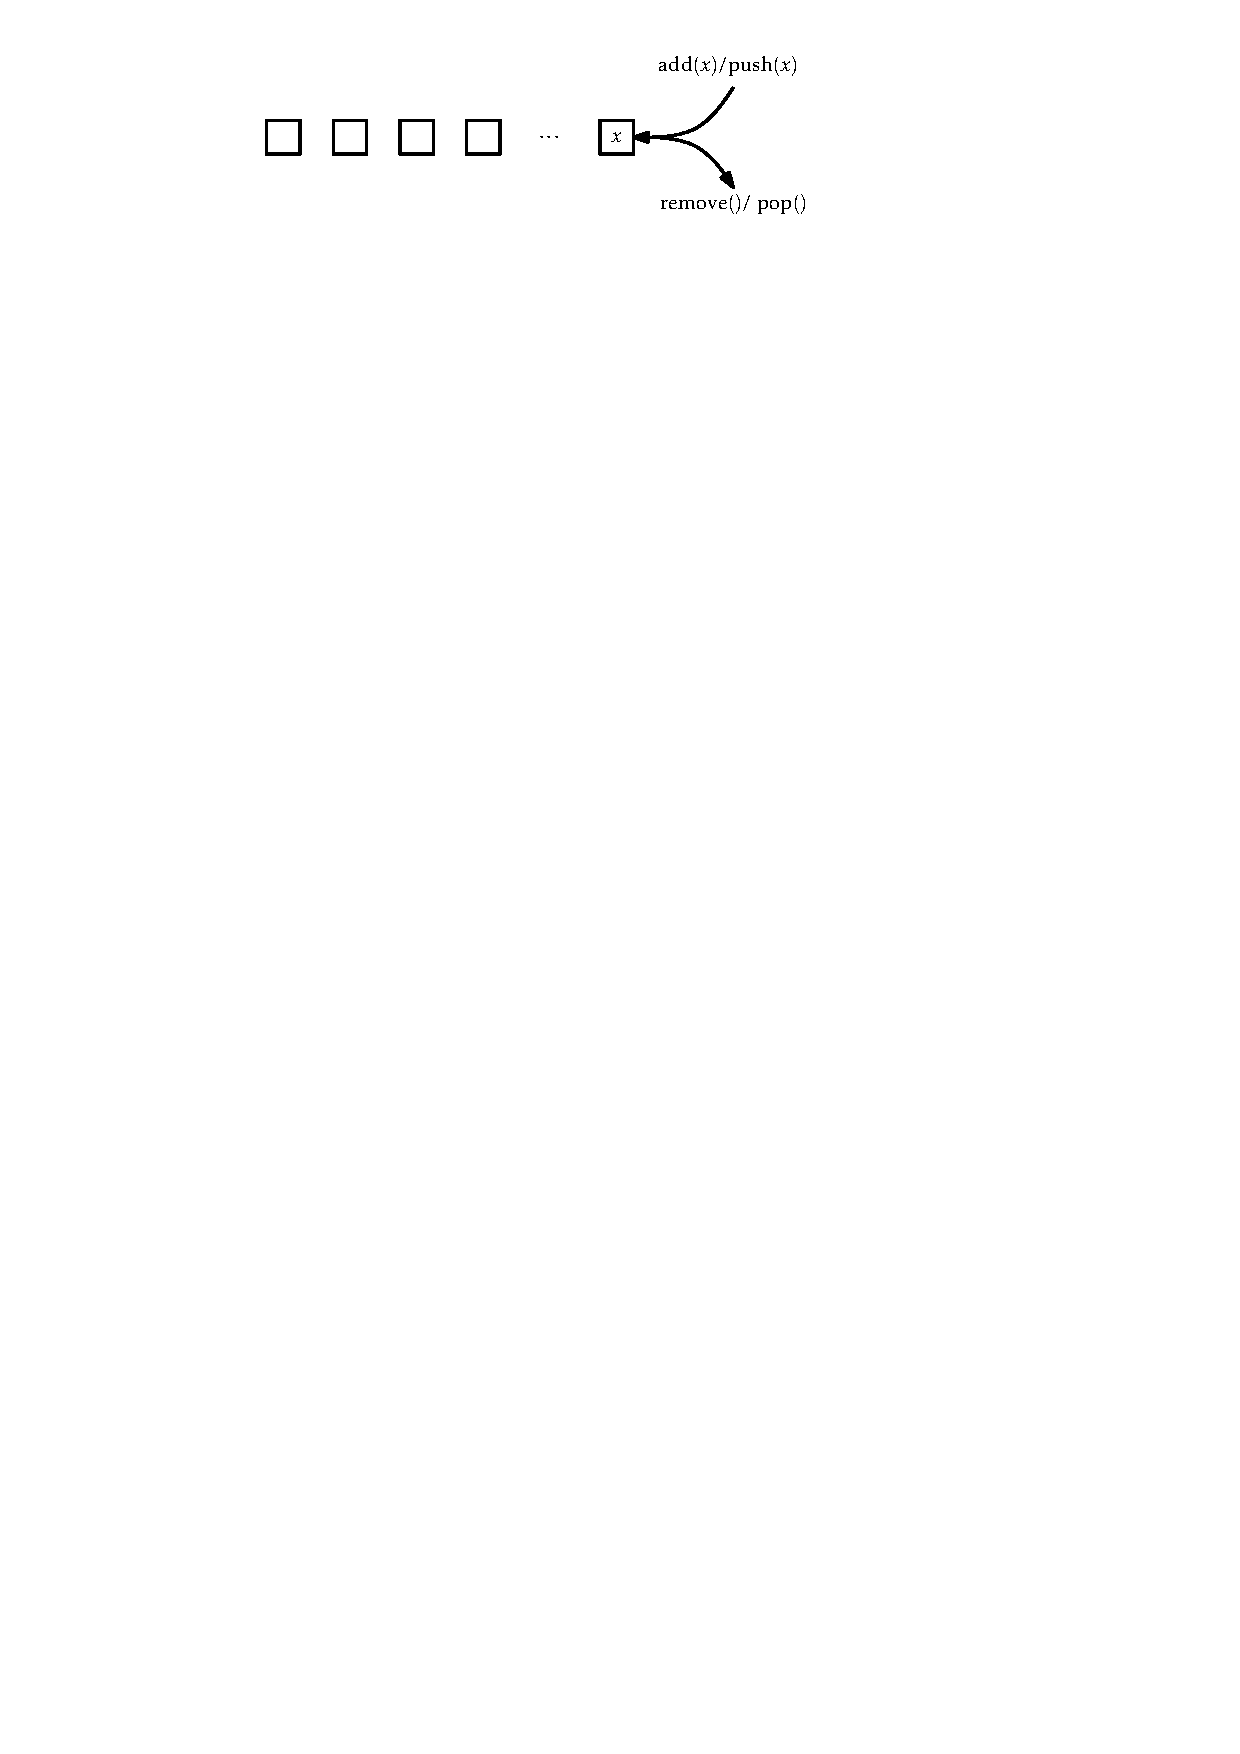
\includegraphics[width=\ScaleIfNeeded]{figs-python/stack}}
	\caption[Uma pilha]{Uma Pilha.}
	\figlabel{stack}
\end{figure}

Uma Deque
\index{deque}%
é uma generalização de ambas #Filas# FIFO e LIFO (#Stack#). Uma #Deque#
representa uma sequência de elementos, com uma frente e uma parte traseira. Os
elementos podem ser adicionados na frente da sequência ou na parte de trás da
sequência. Os nomes das operações de #Deque# são auto-explicativos:
#addFirst(x)#,#removeFirst()#, #addLast(x)# e #removeLast()#. Vale a pena notar
que uma #Pilha# pode ser implementada usando 
apenas #addFirst(x)# e #removeFirst()#, enquanto uma fila FIFO pode ser
implementada usando #addLast(x)# e #removeFirst()#.

\subsection{A interface de #Lista#: sequências lineares}

Este livro falará muito pouco sobre as interfaces #Fila# FIFO, #Pilha# ou
#Deque#. 
Isso ocorre porque essas interfaces são um subconjunto da interface #Lista#. 
Uma #Lista#,
\index{List@List}%
ilustrada na \figref{list}, representa uma sequência, $#x#_0,\ldots,#x#_{#n#-1}$
de valores. A interface #Lista# inclui as seguintes operações:

\begin{enumerate}
	\item #size()#: retorna #n#, o tamanho da lista
	\item #get(i)#: retorna o valor $#x#_{#i#}$
	\item #set(i,x)#: faz o valor de $#x#_{#i#}$ igua a #x#
	\item #add(i,x)#: enfileira #x# na posição #i#, deslocando
	$#x#_{#i#},\ldots,#x#_{#n#-1}$; \\ 
	Faz $#x#_{j+1}=#x#_j$, para todo
	$j\in\{#n#-1,\ldots,#i#\}$, incrementa #n#, e faz $#x#_i=#x#$
	\item #remove(i)# remove o valor $#x#_{#i#}$, deslocando
	$#x#_{#i+1#},\ldots,#x#_{#n#-1}$; \\ 
	Set $#x#_{j}=#x#_{j+1}$, para todo
	$j\in\{#i#,\ldots,#n#-2\}$ e decrementa #n#
\end{enumerate}
Observe que essas operações são mais que suficientes para implementar a
interface #Deque#:
\begin{eqnarray*}
	#addFirst(x)# &\Rightarrow& #add(0,x)# \\
	#removeFirst()# &\Rightarrow& #remove(0)#  \\
	#addLast(x)# &\Rightarrow& #add(size(),x)# \\
	#removeLast()# &\Rightarrow& #remove(size()-1)#
\end{eqnarray*}

\begin{figure}
	\centering{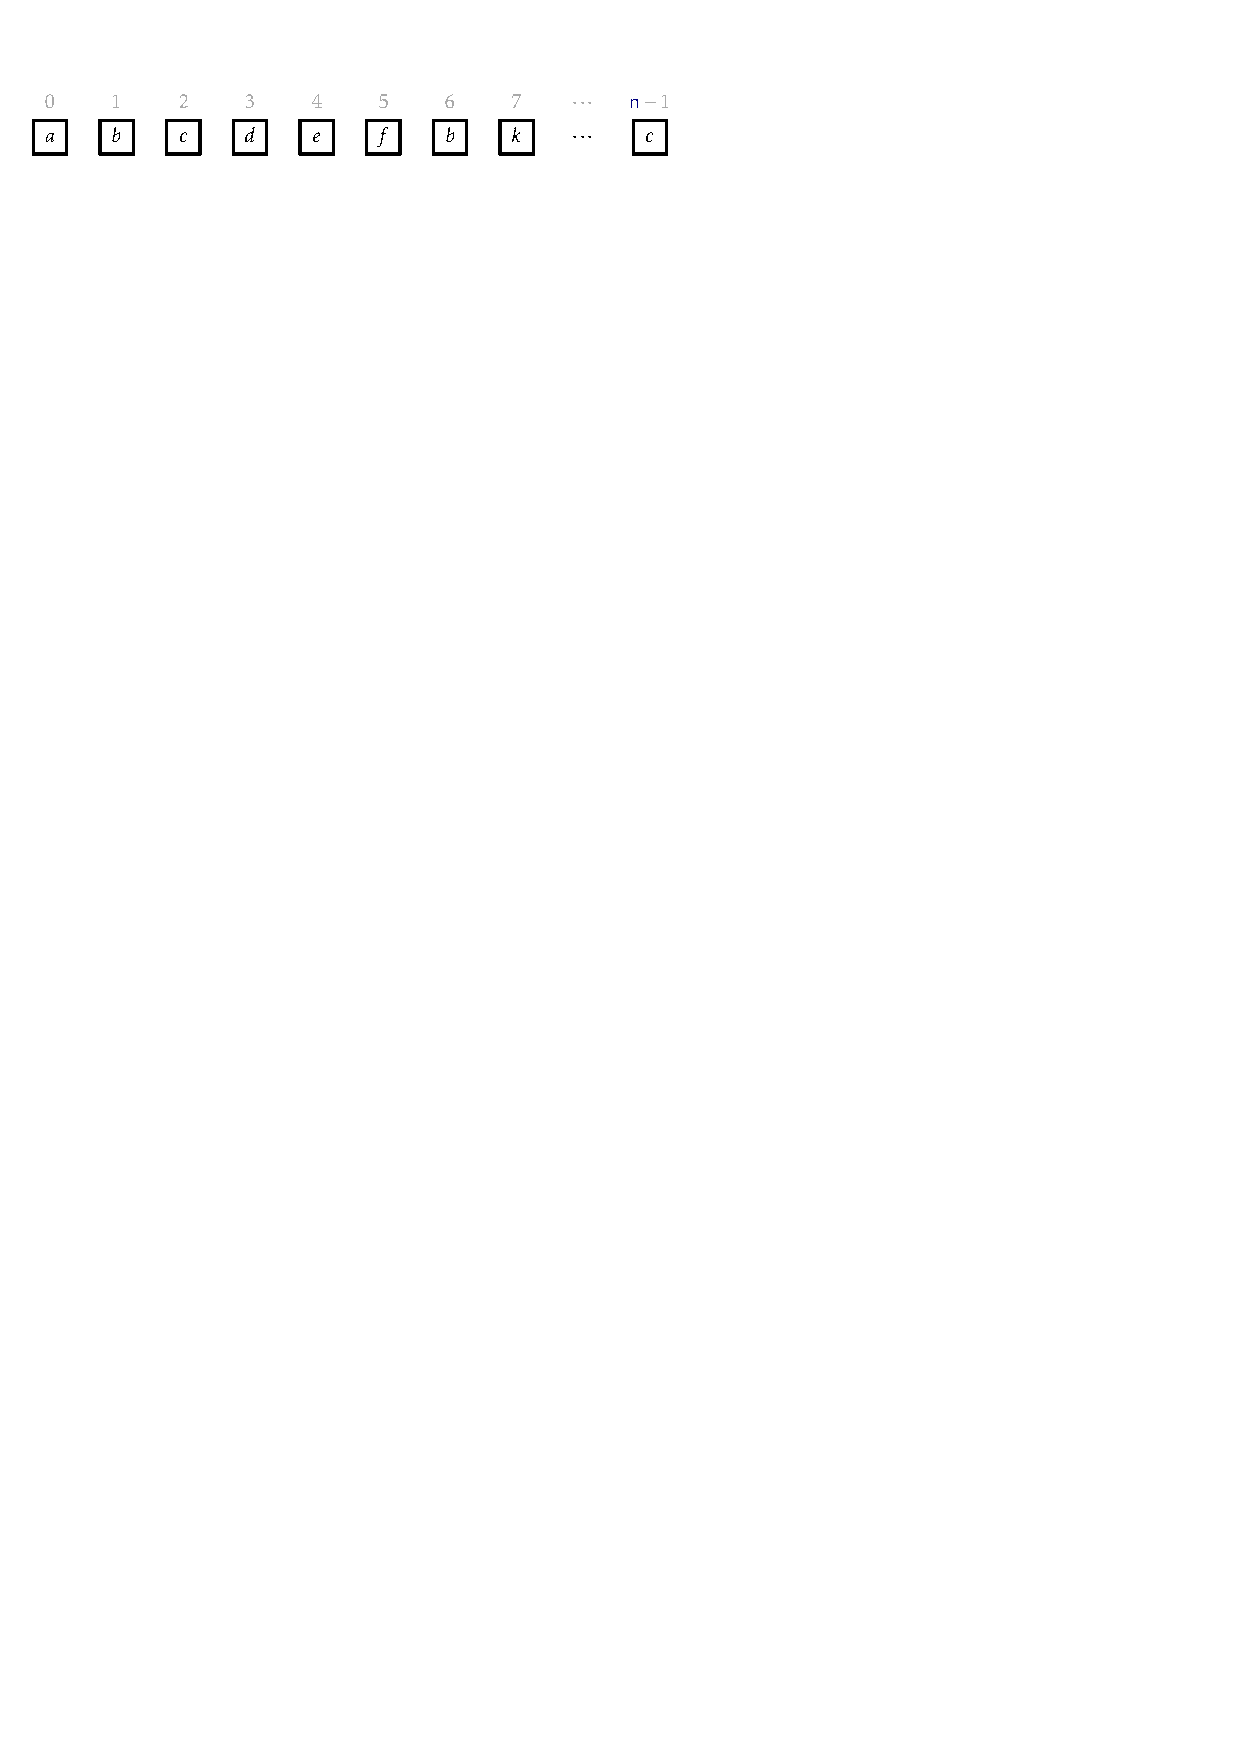
\includegraphics[width=\ScaleIfNeeded]{figs/list}}
	\caption[A List]{Uma Lista representa uma sequência indexada por
		$0,1,2,\ldots,#n#-1$.  Nesta #Lista#, uma chamada para #get(2)# deve retornar		
		o valor $c$.}
	\figlabel{list}
\end{figure}

Embora normalmente não discutamos as interfaces #Pilha#, #Deque# e #Fila# FIFO 
nos capítulos subsequentes, os termos #Pilha# e #Deque# 
às vezes são usados nos nomes das estruturas de dados que implementam a
interface 
#Lista#. Quando isso acontece, destaca o fato de que essas estruturas de dados 
podem ser usadas para implementar a interface #Pilha# ou #Deque# de forma muito 
eficiente. Por exemplo, a classe #ArrayDeque# é uma implementação da interface
#Lista#
que implementa todas as operações #Deque# em tempo constante por operação.

\subsection{A interface #USet#: conjuntos não ordenados}

A interface #USet#
\index{USet@USet}%
representa um conjunto não ordenado de elementos únicos, que imita
a operação matemática \emph{set}. Uma #USet# contém #n# elementos
\emph{distintos}; 
nenhum elemento aparece mais de uma vez; eles não estão em nenhuma ordem
específica.  
Uma #USet# suporta as seguintes operações:

\begin{enumerate}
	\item #size()#: retorna o número, #n#, de elementos no conjunto;
	\item #add(x)#: acrescenta o elemento #x# ao conjunto se ele ainda não estiver
	presente. \\
	Acrescenta #x# ao conjunto desde que não exista nenhum elemento
	#y# no conjunto de tal modo que #x# seja igual a #y#.  Retorna #true#
	se #x# foi acrescentado ao conjunto e #false# caso contrário.
	\item #remove(x)#: remove #x# do conjunto; \\
	Encontra um elemento #y# no conjunto de modo que #x# seja igual a
	#y# e remove #y#.  Retorna #y#, ou #null# se tal elemento não existe.
	\item #find(x)#: encontra #x# no conjunto se ele existe; \\
	Encontra um elemento #y# no conjunto de modo que #y# seja igual a
	#x#.  Retorna #y#, ou #null# se tal elemento não existe.
\end{enumerate}

Essas definições são um pouco exigentes em distinguir #x#, o elemento 
que estamos removendo ou encontrando, de #y#, o elemento que podemos remover ou
encontrar. 
Isso ocorre porque #x# e #y# podem realmente ser objetos distintos que são
tratados como 
iguais. \javaonly{\footnote{Em Java, isso é feito \textit{overriding} os métodos
		#equals(y)# e 
		#hashCode()# da classe.}} Tal distinção é útil porque permite a criação de
\emph{dicionários} 
ou \emph{mapas} que mapeiam chaves em valores.
\index{dicionário}%
\index{map}%

Para criar um dicionário/mapa, formamos objetos compostos chamados #Pares#,
\index{par}%
cada um dos quais contém uma \emph{chave} e um \emph{valor}. Dois #Pares# 
são tratados como iguais se suas chaves são iguais. Se armazenarmos algum par 
$(#k#,#v#)$ em uma #USet# e depois chamamos o método #find(x)# usando o par 
$#x#=(#k#,#null#)$, o resultado será $#y#=(#k#,#v#)$. Em outras palavras, 
é possível recuperar o valor, #v#, dado apenas a chave, #k#.

\subsection{A interface #SSet#: conjuntos ordenados}
\seclabel{sset}

\index{SSet@#SSet#}%
A interface #SSet# representa um conjunto ordenado de elementos. Uma #SSet# 
armazena elementos com algum ordenamento geral, de modo que quaisquer dois elementos
#x# 
e #y# podem ser comparados. Nos exemplos de código, isso será feito com um
método 
chamado #compare(x,y)#, no qual

\[
#compare(x,y)# 
\begin{cases}
{}<0 & \text{se $#x#<#y#$} \\
{}>0 & \text{se $#x#>#y#$} \\
{}=0 & \text{se $#x#=#y#$}
\end{cases}
\]
\index{compare@#compare(x,y)#}%
Uma #SSet# suporta os métodos #size()#, #add(x)# e #remove(x)# com 
a mesma semântica da interface #USet#.  A diferença entre 
uma #USet# e uma #SSet# é o método #find(x)#:
\begin{enumerate}
	\setcounter{enumi}{3}
	\item #find(x)#: localiza #x# no conjunto ordenado; \\
	Encontra o menor elemento #y# no conjunto de modo que $#y# \ge #x#$.
	Retorna #y# ou #null# se tal elemento não existir.
\end{enumerate}

Esta versão da operação #find(x)# é algumas vezes referida como 
uma \emph{busca do sucessor}. %
Ela difere de uma maneira fundamental de 
#USet.find(x)#, uma vez que retorna um resultado significativo, 
mesmo quando não há nenhum elemento igual a #x# no conjunto.

A distinção entre as operações #find(x)# em #USet# e #SSet# é muito 
importante e muitas vezes não é atendida. A funcionalidade adicional 
fornecida por um #SSet# geralmente vem com um preço que inclui tanto 
um maior tempo de execução e uma maior complexidade de implementação. Por
exemplo, na maioria 
das implementações #SSet# discutidas neste livro, todas as operações #find(x)# 
possuem tempos de execução que são logarítmicos de acordo com o tamanho do
conjunto. 
Por outro lado, a implementação de um #USet# como um ChainedHashTable no
\chapref{hashing} 
tem uma operação #find(x)# que é executada em tempo esperado constante. Ao
escolher qual 
dessas estruturas usar, deve-se sempre usar um #USet# a menos que a
funcionalidade 
adicional oferecida por um #SSet# seja realmente necessário.

% \subsection{The DynamicString Interface}

\section{Base Matemática}

Nesta seção, revisamos algumas notações matemáticas e ferramentas usadas ao
longo deste livro, incluindo logaritmos, notação Big-O e teoria de
probabilidade. Esta revisão será breve e não pretende ser uma introdução. Os
leitores que sentem dificuldades com essas bases são encorajados a ler e fazer
exercícios a partir das seções apropriadas do livro excelente (e gratuito) sobre
matemática para a ciência da computação \cite{llm11}.

\subsection{Exponenciais e logaritmos}

\index{exponencial}%
A expressão $b^x$ denota o número $b$ elevado à potência $x$. 
Se $x$ é um inteiro positivo, então este é apenas o valor de $b$ 
multiplicado por si próprio $x-1$ vezes:

\[
b^x = \underbrace{b\times b\times \cdots \times b}_{x} \enspace .
\]
Quando $x$ é um inteiro negativo, $b^{-x}=1/b^{x}$. Quando  $x=0$, $b^x=1$. 
Quando $b$ não é um inteiro, ainda podemos definir a exponenciação em termos 
da função exponencial $e^x$ (ver abaixo), que é, ela própria, definida em 
termos da série exponencial, mas isso é melhor deixar para um texto de cálculo .

\index{logaritmo}%
Neste livro, a expressão $\log_b k $ denota o \emph{logaritmo base $b$} 
de $k$. Ou seja, o valor único $x$ que satisfaz
\[
b^{x} = k  \enspace .
\]
A maioria dos logaritmos neste livro é de base 2 (\emph{logaritmos binários}).
\index{logaritmo binário}%
\index{logaritmo!binário}%
Para estes, omitimos a base, de modo que $\log k$ é abreviação para $\log_2 k$.

Uma maneira informal, porém útil, de pensar em logaritmos, é pensar 
em $\log_b k$ como o número de vezes que temos de dividir $k$ por $b$ 
antes que o resultado seja menor ou igual a 1. Por exemplo, 
quando se faz pesquisa binária, cada comparação reduz o número 
de respostas possíveis por um fator de 2. Isso é repetido até que haja no máximo
uma resposta possível. Portanto, o número de comparação feita por pesquisa
binária quando há inicialmente no máximo $n+1$ respostas possíveis é no máximo
$\lceil\log_2(n+1)\rceil$.

\index{logaritmo natural}%
\index{logaritmo!natural}%
Outro logaritmo que aparece várias vezes neste livro é o \emph{logaritmo
	natural}. 
Aqui usamos a notação $\ln k$ para denotar $\log_e k$, onde $e$ ---
\emph{constante de Euler} --- é dada por
\index{constante de Euler}%
\index{e@$e$ (constante de Euler)}%
\[
e = \lim_{n\rightarrow\infty} \left(1+\frac{1}{n}\right)^n
\approx  2.71828 \enspace .
\]
O logaritmo natural surge frequentemente porque é o valor de uma 
integral particularmente comum:
\[
\int_{1}^{k} 1/x\,\mathrm{d}x  = \ln k \enspace .
\]
Duas das manipulações mais comuns que fazemos com logaritmos são removê-los de
um expoente:
\[
b^{\log_b k} = k
\]
e mudar a base de um logaritmo:
\[
\log_b k = \frac{\log_a k}{\log_a b} \enspace .
\]
Por exemplo, podemos usar essas duas manipulações para comparar os logaritmos
naturais e binários
\[
\ln k = \frac{\log k}{\log e} = \frac{\log k}{(\ln e)/(\ln 2)} = 
(\ln 2)(\log k) \approx 0.693147\log k \enspace .
\]

\subsection{Fatoriais}
\seclabel{factorials}

\index{fatorial}%
Em um ou dois lugares neste livro, a função \emph{fatorial} é usada.
Para um inteiro não negativo $n$, a notação $n!$ (Pronunciada ``$n$ fatorial'')
é definida como significando
\[
n! = 1\cdot2\cdot3\cdot\cdots\cdot n \enspace .
\]
Fatoriais aparecem porque $n!$ conta o número de
permutações, isto é, ordenamentos, de $n$ elementos distintos.
\index{permutacão}%
Para o caso especial $n=0$, $0!$ é definido como 1.

\index{Aproximação de Stirling}%
A quantidade $n!$ pode ser aproximada usando \emph{Aproximação de Stirling}:
\[
n! 
= \sqrt{2\pi n}\left(\frac{n}{e}\right)^{n}e^{\alpha(n)} \enspace ,
\]
onde
\[  
\frac{1}{12n+1} <  \alpha(n) < \frac{1}{12n}  \enspace .
\]
A aproximação de Stirling também aproxima $\ln(n!)$:
\[
\ln(n!) = n\ln n - n + \frac{1}{2}\ln(2\pi n) + \alpha(n)
\]
(De fato, a Aproximação de Stirling é mais facilmente comprovada pela
aproximação
$\ln(n!)=\ln 1 + \ln 2  + \cdots + \ln n$ pela integral
$\int_1^n \ln n\,\mathrm{d}n = n\ln n - n +1$.)

\index{coeficientes binomiais}%
Os \emph{coeficientes binomiais} são relacionadas à função fatorial.
Para um inteiro não-negativo $n$ e um inteiro $k\in\{0,\ldots,n\}$,
a notação $\binom{n}{k}$ indica:
\[
\binom{n}{k} = \frac{n!}{k!(n-k)!} \enspace .
\]
O coeficiente binomial $\binom{n}{k}$ (pronunciado ``$n$ escolhido $k$'')
conta o número de subconjuntos de um conjunto de elementos $n$ que têm o tamanho
$k$,
isto é, o número de maneiras de escolher $k$ inteiros distintos a partir do
conjunto $\{1,\ldots,n\}$.

\subsection{Notação assintótica}

\index{notação assimtótica notation}%
\index{notação big-O }%
\index{notação O@$O$}%
Ao analisar as estruturas de dados neste livro, queremos falar sobre os 
tempos de execução de várias operações. Os tempos de execução exatos, 
naturalmente, variam de computador para computador e até mesmo entre as
execuções 
em um computador individual. Quando falamos sobre o tempo de execução de 
uma operação, estamos nos referindo ao número de instruções do computador 
realizadas durante a operação. Mesmo para o código simples, essa quantidade 
pode ser difícil de calcular exatamente. Portanto, em vez de analisar 
exatamente os tempos de execução, usaremos a chamada  
\emph{notação big-O}: para uma função $f(n)$, $O(f(n))$ denota um conjunto de
funções,
\[
O(f(n)) = \left\{
\begin{array}{l}
g(n):\mbox{existe $c>0$, e $n_0$ tais que} \\
\quad\mbox{$g(n) \le c\cdot f(n)$ para todo $n\ge n_0$}   
\end{array} \right\} \enspace .
\]
Pensando graficamente, este conjunto consiste das funções $g(n)$ onde 
$c\cdot f(n)$ começa a dominar $g(n)$ quando $n$ é suficientemente grande.

Geralmente, utilizamos notação assintótica para simplificar funções. Por
exemplo, 
no lugar de $5n\log n + 8n - 200$ podemos escrever $O(n\log n)$. 
Isto é comprovado da seguinte forma:

\begin{align*} 
5n\log n + 8n - 200
& \le 5n\log n + 8n \\
& \le 5n\log n + 8n\log n & \mbox{ para $n\ge 2$ (então $\log n \ge 1$)}
\\
& \le 13n\log n  \enspace .
\end{align*}
Isso demonstra que a função $f(n)=5n\log n + 8n - 200$  está no 
conjunto $O(n\log n)$ usando as constantes $c=13$ e $n_0 = 2$.

Diversos atalhos úteis podem ser aplicados ao usar notação 
assintótica. Primeiro
\[ O(n^{c_1}) \subset O(n^{c_2}) \enspace ,\]
para qualquer $c_1 < c_2$.  Segundo: para quaisquer constantes $a,b,c > 0$,
\[ O(a) \subset O(\log n) \subset O(n^{b}) \subset O({c}^n) \enspace . \]
Essas relações de inclusão podem ser multiplicadas por qualquer valor positivo, 
e elas ainda são válidas. Por exemplo, a multiplicação por $n$ produz:
\[ O(n) \subset O(n\log n) \subset O(n^{1+b}) \subset O(n{c}^n) \enspace . \]

Continuando em uma longa e distinta tradição, abusaremos desta 
notação escrevendo coisas como $f_1(n) = O(f(n))$ quando o que realmente 
queremos dizer é $f_1(n) \in O(f(n))$. Também faremos declarações como ``o 
tempo de execução desta operação é $O(f(n))$'' quando essa instrução deve 
ser ``o tempo de execução desta operação é \emph{membro de} $O(f(n))$.'' 
Esses atalhos são principalmente para evitar incômodos da linguagem e 
para facilitar a utilização de notação assintótica dentro de cadeias de
equações.

Um exemplo particularmente estranho disso ocorre quando escrevemos
\[
T(n) = 2\log n + O(1)  \enspace .
\]
Novamente, isso seria mais corretamente escrito como
\[
T(n) \le 2\log n + [\mbox{algum membro de $O(1)$]}  \enspace .
\]

A expressão $O(1)$ também traz outra questão. Como não há nenhuma variável 
nessa expressão, pode não estar claro qual variável está ficando 
arbitrariamente grande. Sem contexto, não há maneira de dizer. 
No exemplo acima, uma vez que a única variável no restante da equação 
é $n$, podemos supor que isto deve ser lido como $T(n) = 2\log n + 
O(f(n))$, onde $f(n) = 1$.

A notação Big-O não é algo novo ou exclusivo da ciência da computação. Foi
usada pelo teórico do número Paul Bachmann já em 1894, e é imensamente útil 
para descrever os tempos de execução de algoritmos de computador. 
Considere o seguinte código:
\pcodeimport{ods/Simple.snippet()}
\javaimport{junk/Simple.snippet()}
\cppimport{ods/Simple.snippet()}
Uma execução deste método envolve
\begin{itemize}
	\item $1$ atribuição (\notpcode{#int#}\, #i\, =\, 0#),
	\item $#n#+1$ comparações (#i < n#),
	\item #n# incrementos (#i++#),
	\item #n# cálculos de deslocamentos no vetor (#a[i]#), e
	\item #n# atribuições indiretas (#a[i] = i#).
\end{itemize}
Então, nós poderíamos escrever este tempo de execução como
\[
T(#n#)=a + b(#n#+1) + c#n# + d#n# + e#n# \enspace , 
\]
Onde $a$, $b$, $c$, $d$, e $e$ são constantes que dependem da
máquina que está executando o código e representam o tempo para executar atribuições,
comparações, operações de incremento, cálculos de deslocamento no array e
atribuições, respectivamente. No entanto, se esta expressão representa o
tempo de execução de duas linhas de código, então claramente este tipo de análise
não será tratável para códigos ou algoritmos complicados. Usando a notação big-O,
o tempo de execução pode ser simplificado para
\[
T(#n#)= O(#n#) \enspace .
\]
Não só isso é mais compacto, mas também dá quase tanta informação quanto a expressão
 anterior. O fato de que o tempo de execução depende das constantes $a$, $b$, $c$, $d$ 
 e $e$ no exemplo acima significa que, em geral, não será possível comparar dois tempos 
 de execução para saber qual é mais rápido sem conhecer os valores dessas constantes. 
 Mesmo se fizermos o esforço para determinar essas constantes (digamos, por meio de 
 testes de tempo), então nossa conclusão será válida apenas para a máquina em que 
 executamos nossos testes.

A notação Big-O nos permite raciocinar a um nível muito mais alto, tornando possível analisar funções mais complicadas. Se dois algoritmos tiverem o mesmo tempo de execução big-O, então não saberemos qual é o mais rápido, e pode não haver um vencedor claro. Um pode ser mais rápido em uma máquina, e o outro pode ser mais rápido em uma máquina diferente. No entanto, se os dois algoritmos têm comprovadamente diferentes tempos de execução big-O, então podemos ter certeza de que aquele com menor tempo de execução será mais rápido \emph{para valores suficientemente grandes de #n#}.

Um exemplo de como a notação de big-O nos permite comparar duas funções diferentes é 
mostrado em \figref{intro-asymptotics}, que compara a taxa de crescimento de 
$f_1(#n#)=15#n#$ versus $f_2(n)=2#n#\log#n#$. Pode ser que $f_1(n)$ seja o tempo de execução 
de um algoritmo de tempo linear complicado enquanto $f_2(n)$ é o tempo de execução de um 
algoritmo consideravelmente mais simples baseado no paradigma de divisão e conquista. Isso 
ilustra que, embora $f_1(#n#)$ seja maior que $f_2(n)$ para valores pequenos de #n#,
o oposto é verdadeiro para valores grandes de #n#. Eventualmente $f_1(#n#)$ ganha, por 
uma margem cada vez maior. A análise usando a notação Big-O nos disse que isso aconteceria, 
já que $O(#n#)\subset O(#n#\log #n#)$.

\begin{figure}
	\begin{center}
		\newlength{\tmpa}\setlength{\tmpa}{.98\linewidth}
		\addtolength{\tmpa}{-4mm}
		\resizebox{\tmpa}{!}{\begin{tikzpicture}[gnuplot]
%% generated with GNUPLOT 5.0p3 (Lua 5.1; terminal rev. 99, script rev. 100)
%% Sex 07 Abr 2017 22:14:34 BRT
\path (0.000,0.000) rectangle (12.700,7.620);
\gpcolor{color=gp lt color border}
\gpsetlinetype{gp lt border}
%\gpsetdashtype{gp dt solid}
\gpsetlinewidth{1.00}
\draw[gp path] (1.504,0.985)--(1.684,0.985);
\draw[gp path] (12.147,0.985)--(11.967,0.985);
\node[gp node right] at (1.320,0.985) {$0$};
\draw[gp path] (1.504,1.768)--(1.684,1.768);
\draw[gp path] (12.147,1.768)--(11.967,1.768);
\node[gp node right] at (1.320,1.768) {$200$};
\draw[gp path] (1.504,2.552)--(1.684,2.552);
\draw[gp path] (12.147,2.552)--(11.967,2.552);
\node[gp node right] at (1.320,2.552) {$400$};
\draw[gp path] (1.504,3.335)--(1.684,3.335);
\draw[gp path] (12.147,3.335)--(11.967,3.335);
\node[gp node right] at (1.320,3.335) {$600$};
\draw[gp path] (1.504,4.118)--(1.684,4.118);
\draw[gp path] (12.147,4.118)--(11.967,4.118);
\node[gp node right] at (1.320,4.118) {$800$};
\draw[gp path] (1.504,4.901)--(1.684,4.901);
\draw[gp path] (12.147,4.901)--(11.967,4.901);
\node[gp node right] at (1.320,4.901) {$1000$};
\draw[gp path] (1.504,5.685)--(1.684,5.685);
\draw[gp path] (12.147,5.685)--(11.967,5.685);
\node[gp node right] at (1.320,5.685) {$1200$};
\draw[gp path] (1.504,6.468)--(1.684,6.468);
\draw[gp path] (12.147,6.468)--(11.967,6.468);
\node[gp node right] at (1.320,6.468) {$1400$};
\draw[gp path] (1.504,7.251)--(1.684,7.251);
\draw[gp path] (12.147,7.251)--(11.967,7.251);
\node[gp node right] at (1.320,7.251) {$1600$};
\draw[gp path] (2.472,0.985)--(2.472,1.165);
\draw[gp path] (2.472,7.251)--(2.472,7.071);
\node[gp node center] at (2.472,0.677) {$10$};
\draw[gp path] (3.547,0.985)--(3.547,1.165);
\draw[gp path] (3.547,7.251)--(3.547,7.071);
\node[gp node center] at (3.547,0.677) {$20$};
\draw[gp path] (4.622,0.985)--(4.622,1.165);
\draw[gp path] (4.622,7.251)--(4.622,7.071);
\node[gp node center] at (4.622,0.677) {$30$};
\draw[gp path] (5.697,0.985)--(5.697,1.165);
\draw[gp path] (5.697,7.251)--(5.697,7.071);
\node[gp node center] at (5.697,0.677) {$40$};
\draw[gp path] (6.772,0.985)--(6.772,1.165);
\draw[gp path] (6.772,7.251)--(6.772,7.071);
\node[gp node center] at (6.772,0.677) {$50$};
\draw[gp path] (7.847,0.985)--(7.847,1.165);
\draw[gp path] (7.847,7.251)--(7.847,7.071);
\node[gp node center] at (7.847,0.677) {$60$};
\draw[gp path] (8.922,0.985)--(8.922,1.165);
\draw[gp path] (8.922,7.251)--(8.922,7.071);
\node[gp node center] at (8.922,0.677) {$70$};
\draw[gp path] (9.997,0.985)--(9.997,1.165);
\draw[gp path] (9.997,7.251)--(9.997,7.071);
\node[gp node center] at (9.997,0.677) {$80$};
\draw[gp path] (11.072,0.985)--(11.072,1.165);
\draw[gp path] (11.072,7.251)--(11.072,7.071);
\node[gp node center] at (11.072,0.677) {$90$};
\draw[gp path] (12.147,0.985)--(12.147,1.165);
\draw[gp path] (12.147,7.251)--(12.147,7.071);
\node[gp node center] at (12.147,0.677) {$100$};
\draw[gp path] (1.504,7.251)--(1.504,0.985)--(12.147,0.985)--(12.147,7.251)--cycle;
\node[gp node center,rotate=-270] at (0.246,4.118) {$f({\color{var}\mathtt{n}})$};
\node[gp node center] at (6.825,0.215) {{\color{var}\texttt{n}}};
\node[gp node right] at (10.679,1.627) {$15{\mathtt{n}}$};
\gpcolor{rgb color={0.000,0.376,0.678}}
\gpsetlinewidth{2.00}
\draw[gp path] (10.863,1.627)--(11.779,1.627);
\draw[gp path] (1.504,1.044)--(1.612,1.102)--(1.719,1.161)--(1.827,1.220)--(1.934,1.279)%
  --(2.042,1.337)--(2.149,1.396)--(2.257,1.455)--(2.364,1.514)--(2.472,1.572)--(2.579,1.631)%
  --(2.687,1.690)--(2.794,1.749)--(2.902,1.807)--(3.009,1.866)--(3.117,1.925)--(3.224,1.984)%
  --(3.332,2.042)--(3.439,2.101)--(3.547,2.160)--(3.654,2.219)--(3.762,2.277)--(3.869,2.336)%
  --(3.977,2.395)--(4.084,2.454)--(4.192,2.512)--(4.299,2.571)--(4.407,2.630)--(4.514,2.689)%
  --(4.622,2.747)--(4.729,2.806)--(4.837,2.865)--(4.944,2.924)--(5.052,2.982)--(5.159,3.041)%
  --(5.267,3.100)--(5.374,3.159)--(5.482,3.217)--(5.589,3.276)--(5.697,3.335)--(5.804,3.393)%
  --(5.912,3.452)--(6.019,3.511)--(6.127,3.570)--(6.234,3.628)--(6.342,3.687)--(6.449,3.746)%
  --(6.557,3.805)--(6.664,3.863)--(6.772,3.922)--(6.879,3.981)--(6.987,4.040)--(7.094,4.098)%
  --(7.202,4.157)--(7.309,4.216)--(7.417,4.275)--(7.524,4.333)--(7.632,4.392)--(7.739,4.451)%
  --(7.847,4.510)--(7.954,4.568)--(8.062,4.627)--(8.169,4.686)--(8.277,4.745)--(8.384,4.803)%
  --(8.492,4.862)--(8.599,4.921)--(8.707,4.980)--(8.814,5.038)--(8.922,5.097)--(9.029,5.156)%
  --(9.137,5.215)--(9.244,5.273)--(9.352,5.332)--(9.459,5.391)--(9.567,5.450)--(9.674,5.508)%
  --(9.782,5.567)--(9.889,5.626)--(9.997,5.685)--(10.104,5.743)--(10.212,5.802)--(10.319,5.861)%
  --(10.427,5.919)--(10.534,5.978)--(10.642,6.037)--(10.749,6.096)--(10.857,6.154)--(10.964,6.213)%
  --(11.072,6.272)--(11.179,6.331)--(11.287,6.389)--(11.394,6.448)--(11.502,6.507)--(11.609,6.566)%
  --(11.717,6.624)--(11.824,6.683)--(11.932,6.742)--(12.039,6.801)--(12.147,6.859);
\gpcolor{color=gp lt color border}
\node[gp node right] at (10.679,1.319) {$2{\mathtt{n}}\log{\mathtt{n}}$};
\gpcolor{rgb color={0.867,0.094,0.122}}
\draw[gp path] (10.863,1.319)--(11.779,1.319);
\draw[gp path] (1.504,0.985)--(1.612,1.001)--(1.719,1.022)--(1.827,1.048)--(1.934,1.076)%
  --(2.042,1.106)--(2.149,1.139)--(2.257,1.173)--(2.364,1.208)--(2.472,1.245)--(2.579,1.283)%
  --(2.687,1.322)--(2.794,1.362)--(2.902,1.402)--(3.009,1.444)--(3.117,1.486)--(3.224,1.529)%
  --(3.332,1.573)--(3.439,1.617)--(3.547,1.662)--(3.654,1.707)--(3.762,1.753)--(3.869,1.800)%
  --(3.977,1.847)--(4.084,1.894)--(4.192,1.942)--(4.299,1.991)--(4.407,2.039)--(4.514,2.088)%
  --(4.622,2.138)--(4.729,2.188)--(4.837,2.238)--(4.944,2.289)--(5.052,2.340)--(5.159,2.391)%
  --(5.267,2.443)--(5.374,2.495)--(5.482,2.547)--(5.589,2.600)--(5.697,2.652)--(5.804,2.705)%
  --(5.912,2.759)--(6.019,2.813)--(6.127,2.866)--(6.234,2.921)--(6.342,2.975)--(6.449,3.030)%
  --(6.557,3.085)--(6.664,3.140)--(6.772,3.195)--(6.879,3.251)--(6.987,3.307)--(7.094,3.363)%
  --(7.202,3.419)--(7.309,3.476)--(7.417,3.532)--(7.524,3.589)--(7.632,3.646)--(7.739,3.703)%
  --(7.847,3.761)--(7.954,3.819)--(8.062,3.876)--(8.169,3.934)--(8.277,3.993)--(8.384,4.051)%
  --(8.492,4.110)--(8.599,4.168)--(8.707,4.227)--(8.814,4.286)--(8.922,4.346)--(9.029,4.405)%
  --(9.137,4.464)--(9.244,4.524)--(9.352,4.584)--(9.459,4.644)--(9.567,4.704)--(9.674,4.765)%
  --(9.782,4.825)--(9.889,4.886)--(9.997,4.946)--(10.104,5.007)--(10.212,5.068)--(10.319,5.129)%
  --(10.427,5.191)--(10.534,5.252)--(10.642,5.314)--(10.749,5.375)--(10.857,5.437)--(10.964,5.499)%
  --(11.072,5.561)--(11.179,5.623)--(11.287,5.686)--(11.394,5.748)--(11.502,5.811)--(11.609,5.874)%
  --(11.717,5.936)--(11.824,5.999)--(11.932,6.062)--(12.039,6.126)--(12.147,6.189);
\gpcolor{color=gp lt color border}
\gpsetlinewidth{1.00}
\draw[gp path] (1.504,7.251)--(1.504,0.985)--(12.147,0.985)--(12.147,7.251)--cycle;
%% coordinates of the plot area
\gpdefrectangularnode{gp plot 1}{\pgfpoint{1.504cm}{0.985cm}}{\pgfpoint{12.147cm}{7.251cm}}
\end{tikzpicture}
%% gnuplot variables
}\\[4ex]
		\resizebox{.98\linewidth}{!}{\begin{tikzpicture}[gnuplot]
%% generated with GNUPLOT 5.0p3 (Lua 5.1; terminal rev. 99, script rev. 100)
%% Sex 07 Abr 2017 22:14:34 BRT
\path (0.000,0.000) rectangle (12.700,7.620);
\gpcolor{color=gp lt color border}
\gpsetlinetype{gp lt border}
%\gpsetdashtype{gp dt solid}
\gpsetlinewidth{1.00}
\draw[gp path] (1.872,0.985)--(2.052,0.985);
\draw[gp path] (12.147,0.985)--(11.967,0.985);
\node[gp node right] at (1.688,0.985) {$0$};
\draw[gp path] (1.872,2.029)--(2.052,2.029);
\draw[gp path] (12.147,2.029)--(11.967,2.029);
\node[gp node right] at (1.688,2.029) {$50000$};
\draw[gp path] (1.872,3.074)--(2.052,3.074);
\draw[gp path] (12.147,3.074)--(11.967,3.074);
\node[gp node right] at (1.688,3.074) {$100000$};
\draw[gp path] (1.872,4.118)--(2.052,4.118);
\draw[gp path] (12.147,4.118)--(11.967,4.118);
\node[gp node right] at (1.688,4.118) {$150000$};
\draw[gp path] (1.872,5.162)--(2.052,5.162);
\draw[gp path] (12.147,5.162)--(11.967,5.162);
\node[gp node right] at (1.688,5.162) {$200000$};
\draw[gp path] (1.872,6.207)--(2.052,6.207);
\draw[gp path] (12.147,6.207)--(11.967,6.207);
\node[gp node right] at (1.688,6.207) {$250000$};
\draw[gp path] (1.872,7.251)--(2.052,7.251);
\draw[gp path] (12.147,7.251)--(11.967,7.251);
\node[gp node right] at (1.688,7.251) {$300000$};
\draw[gp path] (2.899,0.985)--(2.899,1.165);
\draw[gp path] (2.899,7.251)--(2.899,7.071);
\node[gp node center] at (2.899,0.677) {$1000$};
\draw[gp path] (3.926,0.985)--(3.926,1.165);
\draw[gp path] (3.926,7.251)--(3.926,7.071);
\node[gp node center] at (3.926,0.677) {$2000$};
\draw[gp path] (4.954,0.985)--(4.954,1.165);
\draw[gp path] (4.954,7.251)--(4.954,7.071);
\node[gp node center] at (4.954,0.677) {$3000$};
\draw[gp path] (5.981,0.985)--(5.981,1.165);
\draw[gp path] (5.981,7.251)--(5.981,7.071);
\node[gp node center] at (5.981,0.677) {$4000$};
\draw[gp path] (7.009,0.985)--(7.009,1.165);
\draw[gp path] (7.009,7.251)--(7.009,7.071);
\node[gp node center] at (7.009,0.677) {$5000$};
\draw[gp path] (8.037,0.985)--(8.037,1.165);
\draw[gp path] (8.037,7.251)--(8.037,7.071);
\node[gp node center] at (8.037,0.677) {$6000$};
\draw[gp path] (9.064,0.985)--(9.064,1.165);
\draw[gp path] (9.064,7.251)--(9.064,7.071);
\node[gp node center] at (9.064,0.677) {$7000$};
\draw[gp path] (10.092,0.985)--(10.092,1.165);
\draw[gp path] (10.092,7.251)--(10.092,7.071);
\node[gp node center] at (10.092,0.677) {$8000$};
\draw[gp path] (11.119,0.985)--(11.119,1.165);
\draw[gp path] (11.119,7.251)--(11.119,7.071);
\node[gp node center] at (11.119,0.677) {$9000$};
\draw[gp path] (12.147,0.985)--(12.147,1.165);
\draw[gp path] (12.147,7.251)--(12.147,7.071);
\node[gp node center] at (12.147,0.677) {$10000$};
\draw[gp path] (1.872,7.251)--(1.872,0.985)--(12.147,0.985)--(12.147,7.251)--cycle;
\node[gp node center,rotate=-270] at (0.246,4.118) {$f({\color{var}\mathtt{n}})$};
\node[gp node center] at (7.009,0.215) {{\color{var}\texttt{n}}};
\node[gp node right] at (10.679,1.627) {$15{\mathtt{n}}$};
\gpcolor{rgb color={0.000,0.376,0.678}}
\gpsetlinewidth{2.00}
\draw[gp path] (10.863,1.627)--(11.779,1.627);
\draw[gp path] (1.872,0.985)--(1.976,1.017)--(2.080,1.049)--(2.183,1.080)--(2.287,1.112)%
  --(2.391,1.144)--(2.495,1.175)--(2.599,1.207)--(2.702,1.238)--(2.806,1.270)--(2.910,1.302)%
  --(3.014,1.333)--(3.117,1.365)--(3.221,1.397)--(3.325,1.428)--(3.429,1.460)--(3.533,1.492)%
  --(3.636,1.523)--(3.740,1.555)--(3.844,1.587)--(3.948,1.618)--(4.052,1.650)--(4.155,1.681)%
  --(4.259,1.713)--(4.363,1.745)--(4.467,1.776)--(4.570,1.808)--(4.674,1.840)--(4.778,1.871)%
  --(4.882,1.903)--(4.986,1.935)--(5.089,1.966)--(5.193,1.998)--(5.297,2.030)--(5.401,2.061)%
  --(5.505,2.093)--(5.608,2.124)--(5.712,2.156)--(5.816,2.188)--(5.920,2.219)--(6.024,2.251)%
  --(6.127,2.283)--(6.231,2.314)--(6.335,2.346)--(6.439,2.378)--(6.542,2.409)--(6.646,2.441)%
  --(6.750,2.473)--(6.854,2.504)--(6.958,2.536)--(7.061,2.567)--(7.165,2.599)--(7.269,2.631)%
  --(7.373,2.662)--(7.477,2.694)--(7.580,2.726)--(7.684,2.757)--(7.788,2.789)--(7.892,2.821)%
  --(7.995,2.852)--(8.099,2.884)--(8.203,2.916)--(8.307,2.947)--(8.411,2.979)--(8.514,3.010)%
  --(8.618,3.042)--(8.722,3.074)--(8.826,3.105)--(8.930,3.137)--(9.033,3.169)--(9.137,3.200)%
  --(9.241,3.232)--(9.345,3.264)--(9.449,3.295)--(9.552,3.327)--(9.656,3.359)--(9.760,3.390)%
  --(9.864,3.422)--(9.967,3.453)--(10.071,3.485)--(10.175,3.517)--(10.279,3.548)--(10.383,3.580)%
  --(10.486,3.612)--(10.590,3.643)--(10.694,3.675)--(10.798,3.707)--(10.902,3.738)--(11.005,3.770)%
  --(11.109,3.802)--(11.213,3.833)--(11.317,3.865)--(11.420,3.896)--(11.524,3.928)--(11.628,3.960)%
  --(11.732,3.991)--(11.836,4.023)--(11.939,4.055)--(12.043,4.086)--(12.147,4.118);
\gpcolor{color=gp lt color border}
\node[gp node right] at (10.679,1.319) {$2{\mathtt{n}}\log{\mathtt{n}}$};
\gpcolor{rgb color={0.867,0.094,0.122}}
\draw[gp path] (10.863,1.319)--(11.779,1.319);
\draw[gp path] (1.872,0.985)--(1.976,1.013)--(2.080,1.050)--(2.183,1.090)--(2.287,1.132)%
  --(2.391,1.175)--(2.495,1.219)--(2.599,1.265)--(2.702,1.311)--(2.806,1.359)--(2.910,1.407)%
  --(3.014,1.455)--(3.117,1.504)--(3.221,1.554)--(3.325,1.604)--(3.429,1.654)--(3.533,1.705)%
  --(3.636,1.756)--(3.740,1.808)--(3.844,1.860)--(3.948,1.912)--(4.052,1.965)--(4.155,2.017)%
  --(4.259,2.071)--(4.363,2.124)--(4.467,2.178)--(4.570,2.232)--(4.674,2.286)--(4.778,2.340)%
  --(4.882,2.395)--(4.986,2.449)--(5.089,2.504)--(5.193,2.560)--(5.297,2.615)--(5.401,2.670)%
  --(5.505,2.726)--(5.608,2.782)--(5.712,2.838)--(5.816,2.894)--(5.920,2.951)--(6.024,3.007)%
  --(6.127,3.064)--(6.231,3.121)--(6.335,3.178)--(6.439,3.235)--(6.542,3.292)--(6.646,3.350)%
  --(6.750,3.407)--(6.854,3.465)--(6.958,3.523)--(7.061,3.581)--(7.165,3.639)--(7.269,3.697)%
  --(7.373,3.755)--(7.477,3.814)--(7.580,3.872)--(7.684,3.931)--(7.788,3.990)--(7.892,4.048)%
  --(7.995,4.107)--(8.099,4.166)--(8.203,4.226)--(8.307,4.285)--(8.411,4.344)--(8.514,4.404)%
  --(8.618,4.463)--(8.722,4.523)--(8.826,4.582)--(8.930,4.642)--(9.033,4.702)--(9.137,4.762)%
  --(9.241,4.822)--(9.345,4.882)--(9.449,4.943)--(9.552,5.003)--(9.656,5.063)--(9.760,5.124)%
  --(9.864,5.185)--(9.967,5.245)--(10.071,5.306)--(10.175,5.367)--(10.279,5.428)--(10.383,5.489)%
  --(10.486,5.550)--(10.590,5.611)--(10.694,5.672)--(10.798,5.733)--(10.902,5.795)--(11.005,5.856)%
  --(11.109,5.917)--(11.213,5.979)--(11.317,6.041)--(11.420,6.102)--(11.524,6.164)--(11.628,6.226)%
  --(11.732,6.288)--(11.836,6.350)--(11.939,6.412)--(12.043,6.474)--(12.147,6.536);
\gpcolor{color=gp lt color border}
\gpsetlinewidth{1.00}
\draw[gp path] (1.872,7.251)--(1.872,0.985)--(12.147,0.985)--(12.147,7.251)--cycle;
%% coordinates of the plot area
\gpdefrectangularnode{gp plot 1}{\pgfpoint{1.872cm}{0.985cm}}{\pgfpoint{12.147cm}{7.251cm}}
\end{tikzpicture}
%% gnuplot variables
}
	\end{center}
	\caption{Gráfico para $15#n#$ versus $2#n#\log#n#$.}
	\figlabel{intro-asymptotics}
\end{figure}

Em alguns casos, usaremos notação assintótica em funções com mais de uma variável. Parece 
não haver um padrão para isso, mas para nossos propósitos, a seguinte definição é suficiente:
\[
O(f(n_1,\ldots,n_k)) = 
\left\{\begin{array}{@{}l@{}}
g(n_1,\ldots,n_k):\mbox{existe $c>0$, e $z$ tal que} \\
\quad \mbox{$g(n_1,\ldots,n_k) \le c\cdot f(n_1,\ldots,n_k)$} \\
\qquad \mbox{para todo $n_1,\ldots,n_k$ tal que
	$g(n_1,\ldots,n_k)\ge z$}   
\end{array}\right\} \enspace .
\]
Esta definição capta a situação que realmente nos interessa: quando os argumentos 
$n_1,\ldots,n_k$ fazem com que $g$ assuma grandes valores. Esta definição também concorda com a 
definição univariada de $O(f(n))$ quando $f(n)$ é uma função crescente de $n$. O leitor deve 
ser advertido que, embora isso funcione para nossos propósitos, outros textos podem tratar 
funções multivariadas e notação assintótica de forma diferente.

\subsection{Randomização e Probabilidade}
\seclabel{randomization}

\index{randomização}%
\index{probabilidade}%
\index{estrutura de dados randomizada}%
\index{algorithm randomizadod}%
Algumas das estruturas de dados apresentadas neste livro são \emph{randomizadas}; elas fazem 
escolhas aleatórias que são independentes dos dados que estão sendo armazenados nelas ou as 
operações que estão sendo realizadas sobre eles. Por esta razão, executar o mesmo conjunto 
de operações mais de uma vez, usando essas estruturas, pode resultar em tempos de execução 
diferentes. Ao analisar essas estruturas de dados, estamos interessados em sua média ou 
tempo de execução \emph{esperado}.
\index{tempo de execução esperado}%
\index{tempo de execução!esperado}%

Formalmente, o tempo de execução de uma operação em uma estrutura de dados aleatória é uma variável aleatória, e queremos estudar seu \emph{valor esperado}. 
\index{valor esperado}%
Para uma variável aleatória discreta $X$ assumindo valores em algum universo contábil $U$, 
o valor esperado de $X$, denotado por $\E[X]$, é dado pela fórmula
\[
\E[X] = \sum_{x\in U} x\cdot\Pr\{X=x\} \enspace .
\]
Aqui $\Pr\{\mathcal{E}\}$ denota a probabilidade de ocorrência do evento 
$\mathcal{E}$. Em todos os exemplos neste livro, essas probabilidades são apenas com relação às escolhas aleatórias feitas pela estrutura de dados randomizados; não há nenhuma suposição de que os dados armazenados na estrutura, ou que a sequência de operações realizadas na estrutura de dados, seja aleatória.

Uma das propriedades mais importantes dos valores esperados é a \emph{linearidade de 
	expectativa}. 
A 
\index {linearidade de expectativa} % 
para quaisquer duas variáveis aleatórias $X$ e $Y$,
\[
\E[X+Y] = \E[X] + \E[Y] \enspace .
\]
De maneira mais geral, para quaisquer variáveis aleatórias $X_1,\ldots,X_k$,
\[
\E\left[\sum_{i=1}^k X_i\right] = \sum_{i=1}^k \E[X_i] \enspace .
\]
A linearidade da expectativa nos permite quebrar variáveis aleatórias complicadas (como os 
lados da esquerda das equações acima) em somas de variáveis aleatórias mais simples (os lados da direita).

Um truque útil, que iremos usar repetidamente, é definir um \emph{indicador de variáveis aleatórias}.
\index{indicador de variáveis aleatórias}%
Estas variáveis binárias são úteis quando queremos contar alguma coisa e são melhor 
ilustradas por um exemplo. Suponha que jogamos uma moeda honesta $k$ vezes e queremos 
saber o número esperado de vezes que a moeda aparece como cara.
\index{lançamento de moedas}%
Intuitivamente, sabemos que a resposta é $k/2$, mas se tentarmos prová-la usando a definição de valor esperado, obtemos
\begin{align*}
\E[X] & = \sum_{i=0}^k i\cdot\Pr\{X=i\} \\
& = \sum_{i=0}^k i\cdot\binom{k}{i}/2^k \\
& = k\cdot \sum_{i=0}^{k-1}\binom{k-1}{i}/2^k \\
& = k/2 \enspace .
\end{align*}
Isso exige que saibamos o suficiente para calcular que $\Pr\{X=i\}
= \binom{k}{i}/2^k$, e que conheçamos as identidades binomiais
$i\binom{k}{i}=k\binom{k-1}{i}$ e $\sum_{i=0}^{k} \binom{k}{i} = 2^{k}$.

Usar indicador de variáveis e linearidade de expectativa torna as coisas muito mais fáceis. Para cada $i\in\{1,\ldots,k\}$, defina o indicador de variável aleatória 
\[
I_i = \begin{cases}
1 & \text{se o $i$-ésimo lançamento de moeda é cara} \\
0 & \text{caso contrário.}
\end{cases}
\]
Então 
\[ \E[I_i] = (1/2)1 + (1/2)0 = 1/2 \enspace . \]
Agora, $X=\sum_{i=1}^k I_i$, so
\begin{align*}
\E[X] & = \E\left[\sum_{i=1}^k I_i\right] \\
& = \sum_{i=1}^k \E[I_i] \\
& = \sum_{i=1}^k 1/2 \\
& = k/2 \enspace .
\end{align*}
Este é um pouco mais longo, mas não requer que nós conheçamos quaisquer 
identidades mágicas ou compute quaisquer probabilidades não triviais. 
Melhor ainda, concorda com a intuição de que esperamos que metade das 
moedas apareça como cara precisamente porque cada moeda individual aparece como cara com
uma probabilidade de $1/2$.

\section{O Modelo de Computação}
\seclabel{model}

Neste livro, analisaremos os tempos teóricos de funcionamento das estruturas de dados 
que estudamos. Para fazer isso precisamente, necessitamos de um modelo matemático 
de computação. Para isso, usamos o modelo de palavra-RAM de \emph{#w#-bits}.
\index{word-RAM}%
\index{RAM} % 
RAM significa Random Access Machine. Neste modelo, temos acesso a uma memória de 
acesso aleatório constituída por \emph{células}, cada uma das quais armazena uma 
\emph{palavra} de #w#-bits. 
\index{palavra}%
Isto implica que uma célula de memória pode representar, por exemplo, qualquer inteiro no conjunto $\{0,\ldots,2^{#w#}-1\}$.

No modelo de palavra-RAM, operações básicas em palavras levam tempo constante.
Isso inclui operações aritméticas (#+#, #-#, #*#, #/#, #%#), 
comparações ($<$, $>$, $=$, $\le$, $\ge$), e operações booleanas bit a bit (AND, OR e exclusivo-OR bit a bit).

Qualquer célula pode ser lida ou escrita em tempo constante. A memória de um computador é 
gerenciada por um sistema de gerenciamento de memória a partir do qual podemos alocar ou 
desalocar um bloco de memória de qualquer tamanho que gostaríamos. Alocar um bloco de 
memória de tamanho $k$ leva um tempo $O(k)$ e retorna uma referência (um ponteiro) para o 
bloco de memória recém-alocado. Esta referência é suficientemente pequena para ser 
representada por uma única palavra.

O tamanho da palavra #w# é um parâmetro muito importante deste modelo. 
O único pressuposto que faremos sobre #w# é o limite inferior $#w# \ge \log #n#$, 
onde #n# é o número de elementos armazenados em qualquer uma das nossas estruturas de dados.
Esta é uma suposição bastante modesta, uma vez que caso contrário uma palavra não é 
mesmo grande o suficiente para contar o número de elementos armazenados na estrutura de dados.

O espaço é medido em palavras, de modo que quando falamos sobre a quantidade de espaço 
usado por uma estrutura de dados, estamos nos referindo ao número de palavras de memória 
usadas pela estrutura. Todas as nossas estruturas de dados armazenam valores de um tipo 
genérico #T#, e assumimos que um elemento do tipo #T# ocupa uma palavra
de memória. \javaonly{(Na realidade, estamos armazenando referências a objetos
do tipo #T#, e essas referências ocupam apenas uma palavra de memória.)}

\javaonly{O modelo de palavra-RAM #w#-bit é relativamente próximo de uma 
	Máquina Virtual Java (JVM) de 32 bits quando $#w#=32$.}\cpponly{O modelo de palavra-RAM de #w#-bit é relativamente próximo dos modernos computadores desktop quando $#w#=32$ ou $#w#=64$.} As estruturas de dados apresentadas neste manual não usam truques especiais que não sejam implementáveis\javaonly{ na JVM e na maioria das outras arquiteturas}\cpponly{ em C++ na maioria das arquiteturas}.

\section{Corretude, Complexidade no Tempo e Complexidade no Espaço}

Ao estudar o desempenho de uma estrutura de dados, há três coisas que mais importam:

\begin{description}
	\item[Corretude:] A estrutura de dados deve implementar corretamente sua interface.
	\index{corretude}%
	\item[Complexidade no Tempo:] Os tempos de execução das operações na estrutura de 
	dados devem ser tão pequenos quanto possível.
	\index{complexidade no tempo}%
	\index{complexidade!time}%
	\item[Complexidade no Espaço:] A estrutura de dados deve usar a menor memória 
	possível.
	\index{complexidade no espaço}%
	\index{complexidade!espaço}%
\end{description}

%Sometimes these three requirements are in conflict with each other. For
%example, it may be possible to have a faster data structure by using
%more space.  It may be possible to have a data structure that is faster,
%or uses less space, if the data structure is allowed to make (hopefully
%occasional) mistakes.

Neste texto introdutório, tomaremos a correção como um dado; não consideraremos estruturas 
de dados que dão respostas incorretas a consultas ou não executam atualizações corretamente. 
Iremos, no entanto, ver estruturas de dados que fazem um esforço extra para manter o uso do 
espaço a um mínimo. Isso normalmente não afeta os tempos de operação (assintóticos) das 
operações, mas pode tornar as estruturas de dados um pouco mais lentas na prática.

Ao estudar tempos de execução no contexto das estruturas de dados, tendemos a obter três 
tipos diferentes de garantias de tempo de execução:

\begin{description}
	\item[Tempo de execução do pior caso:] 
	\index{tempo de execução}%
	\index{tempo de execução!pior caso}%
	\index{tempo de execução para pior caso}%
	Estes são o tipo mais forte de garantias de tempo de execução. Se uma operação 
	de estrutura de dados tiver um pior tempo de execução de $f(#n#)$, então uma dessas
	operações \emph{nunca} demora mais de $f(#n#)$ unidades de tempo.
	\item[Tempo de execução amortizado:]
	\index{tempo de execução!amortizado}%
	\index{tempo de execução amortizado}%
	Se dissermos que o tempo de execução amortizado de uma operação em uma estrutura de 
	dados é $f(#n#)$, então isso significa que o custo de uma operação típica é no máximo 
	$f(#n#)$. Mais precisamente, se uma estrutura de dados tem um tempo de execução 
	amortizado de $f(#n#)$, então uma sequência de $m$ operações leva no máximo 
	$mf(#n#)$ unidades de tempo. Algumas operações individuais podem demorar mais de 
	$f(#n#)$ unidades de tempo, mas a média, ao longo de toda a sequência de operações, é no 
	máximo $f(#n#)$.
	\item[Tempo de execução esperado:] 
	\index{tempo de execução!esperado}%
	\index{tempo de execução esperado}%
	Se dissermos que o tempo de execução esperado de uma operação em uma estrutura de dados 
	é $f(#n#)$, isso significa que o tempo de execução real é uma variável aleatória 
	(ver \secref{randomization}) e o valor esperado desta variável aleatória é no máximo 
	$f(#n#)$. A randomização aqui é com respeito a escolhas aleatórias feitas pela 
	estrutura de dados.
\end{description}

Para entender a diferença entre os tempos de execução de pior caso, amortizado e esperado,
 ajuda considerar um exemplo financeiro. Considere o custo de comprar uma casa:
\paragraph{Pior caso versus custo amortizado:}
\index{custo amortizado}%
Suponha que uma casa custa \$120\,000. Para comprar esta casa, podemos obter uma hipoteca 
de 120 meses (10 anos) com pagamentos mensais de \$1\,200 por mês. Neste caso, o pior caso para o custo mensal de pagar esta hipoteca é \$1\,200 por mês.

Se tivermos dinheiro suficiente à mão, poderemos escolher comprar a casa de uma vez, com um pagamento de \$120\,000. Neste caso, durante um período de 10 anos, o custo mensal amortizado da compra desta casa é
\[
\$120\,000 / 120\text{ meses} = \$1\,000\text{ por mês} \enspace .
\]
Isso é muito menor do que o  \$1\,200 por mês que teríamos que pagar se 
usássemos uma hipoteca.

\paragraph{Pior caso versus custo esperado:}
\index{custo esperado}%
Em seguida, considere a questão do seguro de incêndio em nossa casa de \$120\,000.
Ao estudar centenas de milhares de casos, as companhias de seguros determinaram que a 
quantidade esperada de danos causados por incêndio causados a uma casa como a nossa é 
de \$10 por mês. Este é um número muito pequeno, uma vez que a maioria das casas nunca 
têm incêndios, algumas casas podem ter alguns pequenos incêndios que causam um pouco 
de dano de fumaça, e um pequeno número de casas queimam até suas fundações. Com base 
nestas informações, a companhia de seguros cobra \$15 por mês pelo seguro de incêndio.

Agora é hora da decisão. Deveríamos pagar o custo mensal de \$15 para o seguro de incêndio, 
ou deveríamos apostar e auto-segurar a um custo esperado de \$10 por mês? 
Claramente, o \$10 por mês custa menos \emph{na expectativa}, mas temos que ser capazes 
de aceitar a possibilidade de que o \emph{custo real} pode ser muito maior. No caso 
improvável de que toda a casa queime, o custo real será \$120\,000.

Esses exemplos financeiros também oferecem uma visão sobre porque às vezes nos conformamos 
com um tempo de execução amortizado ou esperado em vez de  um pior tempo de execução.
Muitas vezes é mais provável obter um menor tempo de execução esperado ou amortizado do que 
um pior caso de tempo de execução. Pelo menos, muitas vezes é possível obter uma estrutura 
de dados muito mais simples se estamos dispostos a usar tempos de execução amortizados 
ou esperados.

\section{Exemplos de Código}

\pcodeonly{
	
	Os exemplos de código neste livro são escritos em pseudocódigo.
	\index{pseudocódigo}%
	Estes devem ser fáceis de ler para qualquer pessoa que tenha alguma experiência de 
	programação em qualquer uma das linguagens de programação mais comuns dos últimos 40 anos. 
	Para ter uma ideia de como o pseudocódigo neste livro parece, aqui está uma função que 
	calcula a média de uma matriz, #a#:}
\pcodeimport{ods/Algorithms.average(a)}	
\pcodeonly{	Como esse código ilustra, a atribuição a uma variável é feita usando a notação 
	$\gets$.
	% WARNING: graphic typesetting of assignment operator
	Usamos a convenção de que o tamanho de uma matriz, #a#, é denotado por #len(a)# e os índices de matriz começam em zero, então #range(len(a))# são os índices válidos para 
	#a#. Para encurtar o código, e às vezes torná-lo mais fácil de ler, o nosso pseudocódigo permite atribuições na (sub)matriz. As duas funções a seguir são equivalentes: 
\pcodeimport{ods/Algorithms.left_shift_a(a).left_shift_b(a)}
	O código a seguir define todos os valores de uma matriz como zero:
\pcodeimport{ods/Algorithms.zero(a)}
	Ao analisar o tempo de execução de um código como este, temos de ter cuidado; declarações como
	#a[0:len(a)] = 1#
	ou
	#a[1:len(a)] = a[0:len(a)-1]#
	não executam em tempo constante. Eles são executados em tempo $O(#len(a)#)$.
	
	Tomamos atalhos semelhantes com atribuições de variáveis, de modo que o código 
	#x,y=0,1# define #x# como zero e #y# como 1 e o código #x,y = y,x# troca os valores 
	das variáveis #x# e #y#.
	\index{swap}
	
	Nosso pseudocódigo usa alguns operadores que podem não ser familiares. Como é padrão 
	na matemática, a divisão (normal) é indicada pelo operador $/$.
	Em muitos casos, queremos fazer divisão inteira em vez disso, caso em que usamos o 
	operador $#//#$, de modo que $#a//b# = \lfloor a/b\rfloor$ é a parte inteira de $a/b$.
	Assim, por exemplo, $3/2 = 1.5 $ mas $#3//2# = 1$.
	\index{divisao inteira}%
	\index{operador div}%
	Ocasionalmente, também usamos o operador $\bmod$ para obter o resto da divisão 
	inteira, mas isso será definido quando ele for usado.
	\index{operador mod}%
	\index{operador div}%
	Mais adiante no livro, podemos usar alguns operadores bit a bit, incluindo shift esquerdo (#<<#), shift direito (#>>#), bit a bit e (#&#) e bit a bit exclusivo-ou 
	(#^#).
	\index{left shift}%
	\index{#<<#|see {left shift}}%
	\index{right shift}%
	\index{#>>#|see {right shift}}%
	\index{bitwise and}%
	\index{#&#|see {bitwise and}}%
	\index{#^#|see {bitwise exclusive-or}}%
	
	As amostras de pseudocódigo neste livro são traduções automáticas de código Python que podem ser baixadas do site do livro. \footnote{\url{http://opendatastructures.org}} Se você encontrar uma ambiguidade no pseudocódigo que não possa resolver por si mesmo, então você sempre pode consultar o código Python correspondente. Se você não souber Python, o código também está disponível em Java e C ++. Se você não consegue decifrar o pseudocódigo, ou ler Python, C ++ ou Java, então você pode ainda não estar pronto para este livro.
}

\notpcode{
	Os exemplos de código neste livro são escritos na linguagem de programação \lang. No 
	entanto, para tornar o livro acessível aos leitores não familiarizados com todas as 
	construções e palavras-chave de \lang, as amostras de código foram simplificadas. Por 
	exemplo, um leitor não encontrará nenhuma das palavras-chave #public#, #protected#, 
	#private# ou #static#. Um leitor também não encontrará muita discussão sobre hierarquias 
	de classe. Quais as interfaces que uma determinada classe implementa ou que classe ela 
	estende, se relevante para a discussão, deve ser claro a partir do texto que acompanha.
	
	Estas convenções devem tornar os exemplos de código compreensíveis por qualquer pessoa 
	com uma base em qualquer uma das linguagens da tradição ALGOL, incluindo B, C, C++, 
	C\#, Objective-C, D, Java, Javascript e assim por diante.
	Os leitores que desejam obter detalhes completos de todas as implementações são 
	encorajados a consultar o código fonte \lang\ que acompanha este livro.
	
	Este livro mistura análises matemáticas dos tempos de execução com o código-fonte 
	\lang\ para os algoritmos que estão sendo analisados. Isso significa que algumas 
	equações contêm variáveis também encontradas no código-fonte.
	Essas variáveis são compostas de forma consistente, tanto no código-fonte quanto nas 
	equações. A variável mais comum é a variável #n# 
	\index{n@#n#}% 
	que, sem exceção, sempre se refere ao número de itens atualmente armazenados na 
	estrutura de dados.
}

\section{Lista de Estruturas de Dados}

As tabelas~\ref{tab:summary-i} e \ref{tab:summary-ii} resumem o desempenho das estruturas de 
dados neste livro que implementam cada uma das interfaces, #List#, #USet# e #SSet# descritas em \secref{interfaces}. \Figref{dependencies} mostra as dependências entre vários capítulos 
neste livro.
\index{dependências}%
Uma seta tracejada indica apenas uma dependência fraca, na qual apenas uma pequena parte do 
capítulo depende de um capítulo anterior ou apenas dos principais resultados do capítulo 
anterior.

\begin{table}
	\vspace{56pt}
	\begin{center}
		\resizebox{.98\textwidth}{!}{
			\begin{threeparttable}
				\begin{tabular}{|l|l|l|l|} \hline
					\multicolumn{4}{|c|}{Implementações de #Lista#} \\ \hline
					& #get(i)#/#set(i,x)# & #add(i,x)#/#remove(i)# & \\ \hline
					#ArrayStack# & $O(1)$ & $O(1+#n#-#i#)$\tnote{A} & \sref{arraystack} \\
					#ArrayDeque# & $O(1)$ & $O(1+\min\{#i#,#n#-#i#\})$\tnote{A} & \sref{arraydeque}
					\\
					#DualArrayDeque# & $O(1)$ & $O(1+\min\{#i#,#n#-#i#\})$\tnote{A} &
					\sref{dualarraydeque}\\
					#RootishArrayStack# & $O(1)$ & $O(1+#n#-#i#)$\tnote{A}  &
					\sref{rootisharraystack} \\
					#DLList# & $O(1+\min\{#i#,#n#-#i#\})$ & $O(1+\min\{#i#,#n#-#i#\})$  &
					\sref{dllist} \\
					#SEList# & $O(1+\min\{#i#,#n#-#i#\}/#b#)$ &
					$O(#b#+\min\{#i#,#n#-#i#\}/#b#)$\tnote{A}  & \sref{selist} \\
					#SkiplistList# & $O(\log #n#)$\tnote{E} & $O(\log #n#)$\tnote{E}  &
					\sref{skiplistlist} \\ \hline
					\multicolumn{4}{c}{} \\[2ex] \hline
					\multicolumn{4}{|c|}{Implementações de #USet#} \\ \hline
					& #find(x)# & #add(x)#/#remove(x)# & \\ \hline
					#ChainedHashTable# & $O(1)$\tnote{E} & $O(1)$\tnote{A,E} & \sref{hashtable} \\ 
					#LinearHashTable# & $O(1)$\tnote{E} & $O(1)$\tnote{A,E} & \sref{linearhashtable}
					\\ \hline
				\end{tabular}
				\begin{tablenotes}
					\item[A]{Indica um tempo de execução \emph{amortizado}.}
					\item[E]{Indica um tempo de execução \emph{esperado}.}
				\end{tablenotes}
			\end{threeparttable}}
		\end{center}
		\caption[Sumário das implementações de Lista e USet.]{Sumário das implementações de #Lista# and #USet#.}
		\tablabel{summary-i}
	\end{table}
	
	\begin{table}
		\begin{center}
			\begin{threeparttable}
				\begin{tabular}{|l|l|l|l|} \hline
					\multicolumn{4}{|c|}{Implementações de #SSet#} \\ \hline
					& #find(x)# & #add(x)#/#remove(x)# & \\ \hline
					#SkiplistSSet# & $O(\log #n#)$\tnote{E} & $O(\log #n#)$\tnote{E} &
					\sref{skiplistset} \\ 
					#Treap# & $O(\log #n#)$\tnote{E} & $O(\log #n#)$\tnote{E} & \sref{treap} \\ 
					#ScapegoatTree# & $O(\log #n#)$ & $O(\log #n#)$\tnote{A} & \sref{scapegoattree}
					\\
					#RedBlackTree# & $O(\log #n#)$ & $O(\log #n#)$ & \sref{redblacktree} \\ 
					#BinaryTrie#\tnote{I} & $O(#w#)$ & $O(#w#)$ & \sref{binarytrie} \\ 
					#XFastTrie#\tnote{I} & $O(\log #w#)$\tnote{A,E} & $O(#w#)$\tnote{A,E} &
					\sref{xfast} \\ 
					#YFastTrie#\tnote{I} & $O(\log #w#)$\tnote{A,E} & $O(\log #w#)$\tnote{A,E} &
					\sref{yfast} \\ 
					\javaonly{#BTree# & $O(\log #n#)$ & $O(B+\log #n#)$\tnote{A} & \sref{btree} \\ 
						#BTree#\tnote{X} & $O(\log_B #n#)$ & $O(\log_B #n#)$ & \sref{btree} \\ } \hline
					\multicolumn{4}{c}{} \\[2ex] \hline
					\multicolumn{4}{|c|}{(Priority) Implementações de #Queue#} \\ \hline
					& #findMin()# & #add(x)#/#remove()# & \\ \hline
					#BinaryHeap# & $O(1)$ & $O(\log #n#)$\tnote{A} & \sref{binaryheap} \\ 
					#MeldableHeap# & $O(1)$ & $O(\log #n#)$\tnote{E} & \sref{meldableheap} \\ \hline
				\end{tabular}
				\begin{tablenotes}
					\item[I]{Esta estrutura só pode armazenar dados inteiros de #w#-bit.}
					\javaonly{\item[X]{Isso indica o tempo de execução no modelo de memória externa;;
							see \chapref{btree}.}}
				\end{tablenotes}
				%\renewcommand{\thefootnote}{\arabic{footnote}}
			\end{threeparttable}
		\end{center}
		\caption[Sumário das implementações de SSet e da Fila de prioridade.]{Sumário das implementações de #SSet#
			e da #Fila# de prioridade.}
		\tablabel{summary-ii}
	\end{table}
	
	\begin{figure}
		\begin{center}
			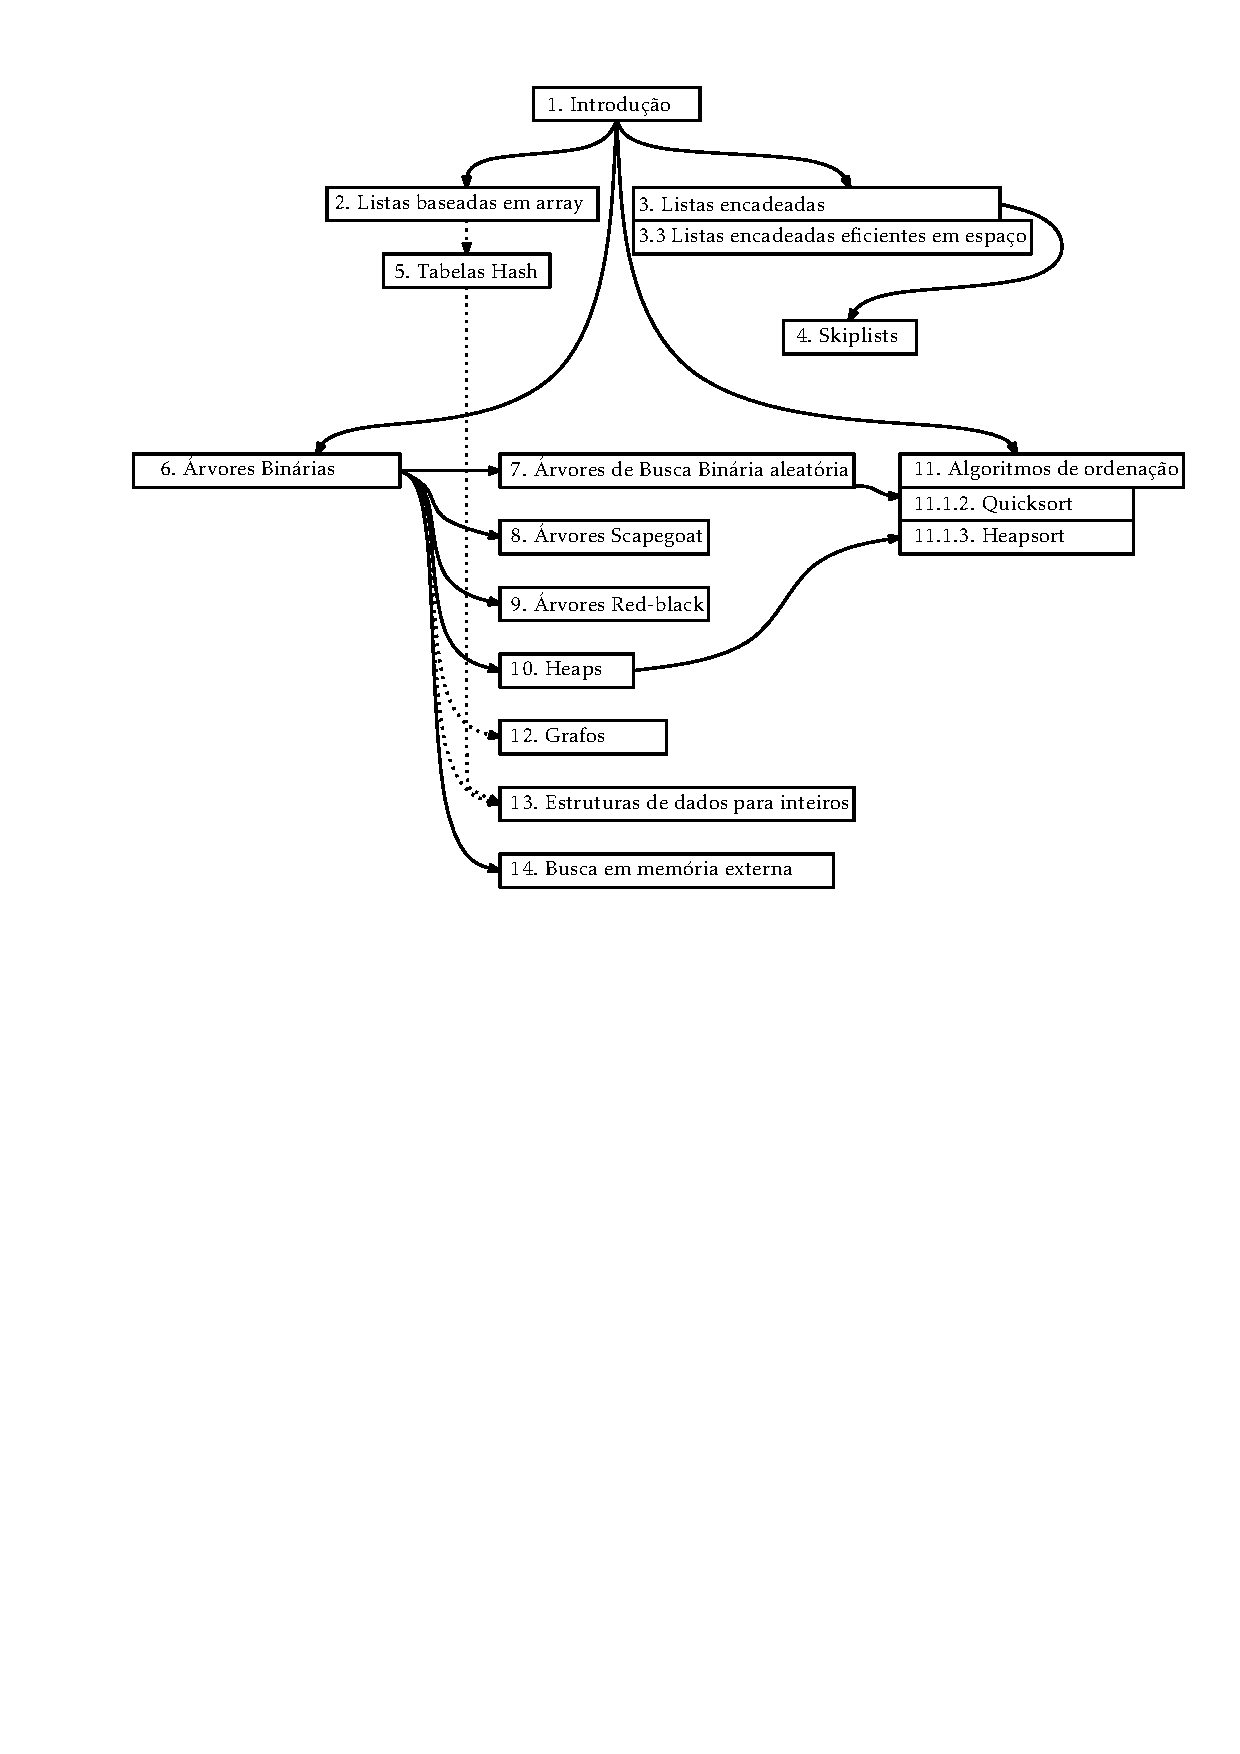
\includegraphics[width=\ScaleIfNeeded]{figs/dependencies}
		\end{center}
		\caption{As dependências entre capítulos neste livro.}
		\figlabel{dependencies}
	\end{figure}
	
	\section{Discussões e Exercícios}
	
	As interfaces #Lista#, #USet# e #SSet# descritas em \secref{interfaces} são 
	influenciadas pelo Framework Java Collections  
	\cite{oracle_collections}.
	\index{Framework Java Collections}%
	Essas são versões essencialmente simplificadas das interfaces #Lista#, #Set#, #Map#, 
	#SortedSet# e #SortedMap# encontradas no Framework Java Collections. \javaonly {O 
		código-fonte que acompanha inclui classes wrapper para fazer implementações de 
		#Uset# e #SSet#  com as implementações de #Set#, #Map#, #SortedSet# e #SortedMap#.}
	
	Para um tratamento soberbo (e livre) da matemática discutido neste capítulo, incluindo 
	a notação assintótica, logaritmos, fatoriais, aproximação de Stirling, probabilidade 
	básica e muito mais, veja o livro de texto de Leyman, Leighton e Meyer \cite{llm11}. 
	Para um texto de cálculo suave que inclui definições formais de exponenciais e 
	logaritmos, veja o texto clássico (livremente disponível) por Thompson \cite{t14}.
	
	Para obter mais informações sobre probabilidade básica, especialmente no que se refere à 
	ciência da computação, consulte o livro de texto de Ross \cite{r01}. Outra boa 
	referência, que abrange tanto a notação assintótica quanto a probabilidade, é o 
	livro de Graham, Knuth e Patashnik \cite{gkp94}.
	
	\javaonly{Os leitores que querem aperfeiçoar sua programação de Java podem encontrar muitos tutorials de Java em linha em \cite{oracle_tutorials}.}
	
	\begin{exc}
		Este exercício foi projetado para ajudar a familiarizar o leitor com a escolha da 
		estrutura de dados correta para o problema correto. Se implementado, as partes deste 
		exercício devem ser feitas usando uma implementação da interface relevante (#Stack#,
		 #Queue#, #Deque#, #USet# ou #SSet#)\javaonly{ fornecida pelo Framework Java Collections }\cpponly{ fornecida pelo C++ Standard Template Library}.
		
		Resolva os seguintes problemas lendo um arquivo de texto uma linha por vez e 
		executando operações em cada linha na(s) estrutura(s) de dados apropriada(s). Suas 
		implementações devem ser rápidas o suficiente para que mesmo arquivos contendo um 
		milhão de linhas possam ser processados em poucos segundos.
		\begin{enumerate}
			\item Leia a entrada de uma linha de cada vez e, em seguida, escreva as linhas 
			em ordem inversa, de modo que a última linha de entrada seja impressa primeiro,
			depois a segunda última linha de entrada, e assim por diante.
			
			\item  Leia as primeiras 50 linhas de entrada e depois escreva-as em ordem 
			inversa. Leia as próximas 50 linhas e depois escreva-as em ordem inversa. Faça 
			isso até que não haja mais linhas deixadas para ler, neste ponto, quaisquer 
			linhas restantes devem ser impressas na ordem inversa.
			
			Em outras palavras, sua saída começará com a 50ª linha, depois com a 49ª, 
			depois com a 48ª, e assim por diante até a primeira linha. Isto será 
			seguido pela 100ª linha, seguida pela 99ª, e assim por diante até a 51ª. O processo continua indefinidamente.
			
			Seu código nunca deve ter que armazenar mais de 50 linhas em um determinado 
			momento.
			
			\item Leia a entrada uma linha de cada vez.
			Em qualquer ponto depois de ler as primeiras 42 linhas, se alguma linha estiver 
			em branco (ou seja, uma sequência de comprimento 0), imprima a linha que ocorreu 
			42 linhas anteriores a essa. Por exemplo, se a Linha 242 estiver em branco, 
			então seu programa deve imprimir a linha 200. Este programa deve ser 
			implementado de modo que nunca armazene mais de 43 linhas da entrada a qualquer 
			momento.
			
			\item Leia a entrada uma linha de cada vez e escreva cada linha na saída se não for uma duplicata de alguma linha de entrada anterior. Tome especial cuidado para que um arquivo com um monte de linhas duplicadas não use mais memória do que o necessário para o número de linhas únicas.
			
			\item Leia a entrada uma linha de cada vez e escreva cada linha para a saída somente se você já leu esta linha antes. (O resultado final é que você remove a primeira ocorrência de cada linha.)
			Tome especial cuidado para que um arquivo com um monte de linhas duplicadas não use mais memória do que o necessário para o número de linhas únicas.
			
			\item Leia toda a entrada uma linha de cada vez. Em seguida, imprima todas as 
			linhas ordenadas por comprimento, com as linhas mais curtas primeiro. No caso em 
			que duas linhas tenham o mesmo comprimento, resolva sua ordem usando a ``ordem classificada''. As linhas duplicadas devem ser impressas apenas uma vez.
			
			\item Faça o mesmo que a pergunta anterior, exceto que as linhas duplicadas devem ser impressas o mesmo número de vezes que aparecem na entrada.
			
			\item Leia toda a entrada uma linha de cada vez e, em seguida, imprimir as linhas pares numeradas (começando com a primeira linha, linha 0) seguida pelas linhas ímpares.
			
			\item Leia toda a entrada uma linha de cada vez e permute aleatoriamente as linhas antes de imprimi-las. Para ser claro: Você não deve modificar o conteúdo de qualquer linha. Em vez disso, a mesma coleção de linhas deve ser impressa, mas em uma ordem aleatória....
		\end{enumerate}
	\end{exc}
	
	\begin{exc}
		\index{Palavra de Dyck}%
		Uma \emph{palavra Dyck } é uma sequência de +1's e -1's com a propriedade que
		a soma de qualquer prefixo da sequência nunca seja negativo.  
		Por exemplo,
		$+1,-1,+1,-1$ é uma palavra \textit{Dyck}, porém $+1,-1,-1,+1$ não é uma palavra \textit{Dyck} posto
		que o prefixo $+1-1-1<0$.  Descreva qualquer relação entre palavras Dyck e as operações na #Stack# #push(x)# e #pop()#.
	\end{exc}
	
	\begin{exc}
		\index{string casada}%
		\index{string!casada}%
		Uma \emph{string casada} é uma sequência de caracteres \{, \}, (, ), [, e ]
		que estão casados de forma correta.  Por exemplo, ``\{\{()[]\}\}''
		é uma string casada, porém ``\{\{()]\}'' não é, posto que o segundo \{
		casa com um ].  Mostre como usar uma pilha para que, dada uma string
		de comprimento #n#, você possa determinar se ela é uma string casada em um
		tempo $O(#n#)$.
	\end{exc}
	
	\begin{exc}
		Suponha que você tenha uma #Stack#, #s#, que suporta somente as operações 
		#push(x)# e #pop()#. Mostre como, usando apenas uma #Fila# FIFO, #f#, você pode 
		inverter a ordem de todos os elementos em #s#.
	\end{exc}
	
	\begin{exc}
		\index{Bag@#Bag#}%
		Usando um #USet#, implementar um #Bag#. Um #Bag# é como um #USet# --- suporta os métodos #add(x)#, #remove(x)# e #find(x)# mas permite que elementos duplicados sejam 
		armazenados. A operação #find(x)# em um #Bag# retorna algum elemento (se houver) 
		que é igual a #x#. Além disso, um #Bag# suporta a operação #findAll(x)# 
		que retorna uma lista de todos os elementos no #Bag# que são iguais a #x#.
		\end{exc}
	
	\begin{exc}
		A partir do zero, escreva e teste as implementações das interfaces #Lista#, #USet# 
		e #SSet#. Estas não têm de ser eficientes. Elas podem ser usados mais tarde para testar a correção e o desempenho de implementações mais eficientes. (A maneira 
		mais fácil de fazer isso é armazenar os elementos em uma matriz.)
	\end{exc}
	
	\begin{exc}
		Trabalhe para melhorar o desempenho de suas implementações a partir da pergunta anterior usando quaisquer truques que você possa pensar. Experimente e pense sobre como você poderia melhorar o desempenho de #add(i,x)# e #remove(i)# em sua 
		implementação #Lista#. Pense em como você poderia melhorar o desempenho da operação 
		#find(x)# em suas implementações de #USet# e #SSet#. Este exercício é projetado para dar-lhe uma sensação de como é difícil obter implementações eficientes dessas 
		interfaces.
	\end{exc}
	
	
	
	
	
